\documentclass[tocnosub,noragright,centerchapter,12pt]{uiucecethesis09}
    % \documentclass[draftthesis,tocnosub,noragright,centerchapter,12pt]{uiucecethesis09}

% Use draftthesis for notes and date markings on every page.  Useful when you
%   have multiple copies floating around.
% Use offcenter for the extra .5 inch on the left side. Needed with fullpage and fancy.
% Use mixcasechap for compatibility with hyperref package, which does NOT like all caps default
% Use edeposit for the adviser/committee on the title page.
% Use tocnosub to suppress subsection and lower entries in the TOC.
% PhD candidates use "proquest" for the proquest abstract.

\makeatletter

% \usepackage[titlenumbered,ruled]{algorithm2e}
\usepackage{algorithm}
\usepackage{algpseudocode}
\usepackage{amsfonts}
\usepackage{amsmath}  % for math spacing
\usepackage[page]{appendix}
\usepackage{array}
\usepackage{bm}
\usepackage[justification=raggedright]{caption}	% makes captions ragged right - thanks to Bryce Lobdell
\usepackage{color}
% \usepackage{epsfig}  % for figures
\usepackage{graphicx}  % another package that works for figures
% \usepackage[hidelinks]{hyperref}
% \hypersetup{
%     colorlinks,
%     allcolors=black,
%     % citecolor=black,
%     % filecolor=black,
%     % linkcolor=black,
%     % urlcolor=black
% }
% \usepackage{subfigure}  % for subfigures
%\usepackage{amssymb}  % for math spacing
%\usepackage{url}  % Hyphenation of URLs.
\usepackage{listings}
\usepackage{lscape}  % Useful for wide tables or figures.
\usepackage{makecell}
\usepackage{microtype}
\usepackage{setspace}
\usepackage{subcaption}
\usepackage{tabularx}
\usepackage{varwidth}

% Fix long URL line breaks in bibliography
\usepackage{url}
\def\UrlBreaks{\do\/\do-}

\lstset{basicstyle=\footnotesize\ttfamily,
        keywordstyle=\color{blue}\ttfamily,
        stringstyle=\color{red}\ttfamily,
        commentstyle=\color{green}\ttfamily,
        morecomment=[l][\color{magenta}]{\#}
}


\usepackage{svg}
% \usepackage{tikz}
% \usetikzlibrary{arrows}
% \usetikzlibrary{positioning}
% \usetikzlibrary{arrows.meta}



\newcommand{\mytilde}{\raise.17ex\hbox{$\scriptstyle\mathtt{\sim}$}}
\newcolumntype{P}[1]{>{\centering\arraybackslash}p{#1}}
\newcolumntype{M}[1]{>{\centering\arraybackslash}m{#1}}
\newcolumntype{Y}{>{\centering\arraybackslash}X}


\newif\ifsubmit
% \submittrue
\submitfalse
\ifsubmit

    \newcommand{\todo}[1]{}
    \newcommand{\tocite}[1]{}
    \newcommand{\outline}[1]{}
    \newcommand{\addtext}[1]{#1}
    \newcommand{\rmtext}[1]{}

\else

    \definecolor{commentColor}{rgb}{0.1, 0.6, 1.0}
    \definecolor{outlineColor}{rgb}{0.0, 0.50, 0.0}
    \definecolor{toCiteColor}{rgb}{0.5, 0.0, 0.5}
    \definecolor{addedColor}{rgb}{0.3, 0.5, 1.0}
    \definecolor{removedColor}{rgb}{0.8, 0.8, 0.8}

    \newcommand{\todo}[1]{[{\color{red}TODO: #1}]}
    \newcommand{\tocite}[1]{[{\color{toCiteColor}CITE: #1}]}
    \newcommand{\outline}[1]{[{\color{outlineColor}OUTLINE: #1}]}
    \newcommand{\addtext}[1]{{\color{addedColor}#1}}
    \newcommand{\rmtext}[1]{{\color{removedColor}\sout{#1}}}

\fi

% Number algorithms by chapter
\renewcommand{\thealgorithm}{\arabic{chapter}.\arabic{algorithm}} 

% Uncomment the appropriate one of the following four lines:
\msthesis
%\phdthesis
%\otherdoctorate[abbrev]{Title of Degree}
%\othermasters[abbrev]{Title of Degree}

\title{Heterogeneous System and Application Communication Modeling}
\author{Carl Pearson}
\department{Electrical and Computer Engineering}
\degreeyear{2018}

% Advisor name is required for
% - doctoral students for the ProQuest abstract
% - master's students who do not have a master's committee
\advisor{Professor Wen-Mei Hwu}

% Uncomment the \committee command for
% - all doctoral students
% - master's students who have a master's committee
%\committee{Professor Firstname Lastname, Chair\\
%        Professor Firstname Lastname} % etc.

\begin{document}

%%%%%%%%%%%%%%%%%%%%%%%%%%%%%%%%%%%%%%%%%%%%%%%%%%%%%%%%%%%%%%%%%%%%%%%%%%%%%%%
% COPYRIGHT
%
%\copyrightpage
%\blankpage

%%%%%%%%%%%%%%%%%%%%%%%%%%%%%%%%%%%%%%%%%%%%%%%%%%%%%%%%%%%%%%%%%%%%%%%%%%%%%%%
% TITLE
%
\maketitle

%\raggedright
\parindent 1em%

\frontmatter

%%%%%%%%%%%%%%%%%%%%%%%%%%%%%%%%%%%%%%%%%%%%%%%%%%%%%%%%%%%%%%%%%%%%%%%%%%%%%%%
% ABSTRACT
%
\begin{abstract}
	% Put the abstract in a file called "abs.tex" and it'll be inputted here.
	With the end of dennard scaling, high-performance computing increasingly relies on heterogeneous systems with specialized hardware to improve application performance.
This trend has driven up the complexity of high-performance software development, as developers must manage multiple programming systems and develop system-tuned code to utilize specialized hardware.
In addition, it has exacerbated existing challenges of data placement as the specialized hardware often has local memories to fuel its computational demands.
In addition to using appropriate software resources to target application computation at the best hardware for the job, application developers now much manage data movement and placement within their application, which also must be specifically tuned to the target system.
Instead of relying on the application developer to have specialized knowledge of system characteristics and specialized expertise in multiple programming systems, this work proposes a heterogeneous system communication library that automatically choses data location and data movement for high-performance application development and execution on heterogeneous systems.
This work presents the foundational components of that library: a systematic approach for characterization of system communication links and application communication demands.
\end{abstract}


%%%%%%%%%%%%%%%%%%%%%%%%%%%%%%%%%%%%%%%%%%%%%%%%%%%%%%%%%%%%%%%%%%%%%%%%%%%%%%%
% DEDICATION
%
\begin{dedication}
	% Whatever dedication you want.
	To my family, for their love and support.
\end{dedication}

%%%%%%%%%%%%%%%%%%%%%%%%%%%%%%%%%%%%%%%%%%%%%%%%%%%%%%%%%%%%%%%%%%%%%%%%%%%%%%%
% ACKNOWLEDGMENTS
%
% Put acknowledgments in a file called "ack.tex" and it'll be inputted here.
\begin{acknowledgments}
	I would like to thank Professor Wen-Mei Hwu.

I would also like to thank the members of the IMPACT group for their continual support.
\end{acknowledgments}

%%%%%%%%%%%%%%%%%%%%%%%%%%%%%%%%%%%%%%%%%%%%%%%%%%%%%%%%%%%%%%%%%%%%%%%%%%%%%%%
% TABLE OF CONTENTS
%
\tableofcontents

%%%%%%%%%%%%%%%%%%%%%%%%%%%%%%%%%%%%%%%%%%%%%%%%%%%%%%%%%%%%%%%%%%%%%%%%%%%%%%%
% LIST OF TABLES
%
% The List of Tables is not strictly necessary. Omitting the List of Tables will
% simplify the thesis check and reduce the number of corrections.
\listoftables

%%%%%%%%%%%%%%%%%%%%%%%%%%%%%%%%%%%%%%%%%%%%%%%%%%%%%%%%%%%%%%%%%%%%%%%%%%%%%%%
% LIST OF FIGURES
%
% The List of Figures is not strictly necessary. Omitting the List of Figures will
% simplify the thesis check and reduce the number of corrections.
\listoffigures

\renewcommand\lstlistlistingname{LIST OF CODE LISTINGS}
\clearpage
\addcontentsline{toc}{chapter}{\lstlistlistingname}
\lstlistoflistings

\clearpage
\addcontentsline{toc}{chapter}{LIST OF ALGORITHMS}
\listofalgorithms



%%%%%%%%%%%%%%%%%%%%%%%%%%%%%%%%%%%%%%%%%%%%%%%%%%%%%%%%%%%%%%%%%%%%%%%%%%%%%%%
% LIST OF ABBREVIATIONS
%
% The List of Abbreviations is not strictly necessary.
\chapter{LIST OF ABBREVIATIONS}

\begin{symbollist*}
	\item[CUDA] Compute Unified Device Architecture
	\item[FPGA] field-programmable gate array
	\item[GPU] graphics processing unit
	\item[NUMA] Non-uniform memory access
	\item[RAM] random-access memory
	\item[SIMD] single-instruction multiple-data
	\item[SMP] symmetric multi-processing
\end{symbollist*}


%%%%%%%%%%%%%%%%%%%%%%%%%%%%%%%%%%%%%%%%%%%%%%%%%%%%%%%%%%%%%%%%%%%%%%%%%%%%%%%
% LIST OF SYMBOLS
%
% \begin{symbollist}[0.7in]
	% \item[$G_a$] application graph
	% \item[$G_s$] system graph
% \end{symbollist}

\mainmatter

%%%%%%%%%%%%%%%%%%%%%%%%%%%%%%%%%%%%%%%%%%%%%%%%%%%%%%%%%%%%%%%%%%%%%%%%%%%%%%%
% INSERT REAL CONTENT HERE
%


\chapter{Introduction}
Add a citation~\cite{IEEEexample:urlsty} to make the build not fail.

The first chapter should introduce the problem studied and describe the main results obtained in the thesis.
In order to provide guidance to the reader, the first chapter should briefly describe the organization of the rest of the thesis.
The first chapter can also give the background of previous work on the subject and the method used in attacking the problem.
\chapter{Background}


%
%
%
\section{Communication Links}

\subsection{PCI}
\subsection{NVLink}
\subsection{QPI}
\subsection{X bus}
\subsection{CAPI}

%
%
%
\section{Programming Systems}
\subsection{CUDA}
\label{sec:cuda}


CUDA Unified Memory~\cite{harris2013cudaunifiedmemory} provides a single pool of memory that is accessible from the CPU and GPU by a single pointer.
CUDA automatically migrates data between the physically distinct CPU and GPU memory as needed, allowing GPU kernels to access the memory as if it were in the global memory, and CPU functions to access the memory as if it were in the system memory.
This simplifies the programming model.

\todo{unified memory peer access}

\subsection{HSA}
\label{sec:hsa}


%
%
%
\section{Profiling Tooling}

\subsection{CUDA Profiling Tools Interface}
\label{sec:cupti}

The CUDA Profiling Tools Interface~\cite{nvidia2017cupti} (CUPTI) ``provides...detailed information about how applications are using the GPU in a system.''
Users may inject code into the entry and exit point of every CUDA C Runtime and CUDA Driver API function call.
Additionally, users may configure and query hardware and software event counters to get insight into the operation of the GPU and CUDA stack.
The event counters include instruction count, instruction throughput, memory loads/stores, memory throughput, cache hits/misses, branches and custom profile triggers.
Chapter~\ref{ch:app-char} describes how \todo{hwcomm-apptracer} uses CUPTI to record memory allocations, kernel arguments, and timestamps to build a model of the application execution.

\subsection{\texttt{LD\_PRELOAD}}
\label{sec:ldpreload}

LD\_PRELOAD~\cite{kerrisk2017ld} is a mechanism by which the ld linker will load additional user-specific shared objects before any others.
If a function definition is present in a pre-loaded shared object, it will override the implementation present in later objects.
When combined with dlsym()~\cite{kerrisk2017dlysm}, it can be used to inject code into the entry of library calls in dynamically-linked binaries.
Chapter~\ref{ch:app-char} describes how \todo{hwcomm-apptracer} uses LD\_PRELOAD to record special information about cuBLAS and cuDNN calls.

\cite{kerrisk2017ld}


\chapter{System Characterization}
\label{ch:sys-char}

High-performance data movement in heterogeneous systems requires information about the properties of the communication links between system storage and compute components.
Although specifications of system components are often available\todo{cite some examples}, the real-world properties of these links depends on how applications use the links, and whether or not the links are shared between system components.
\todo{For example, Figure~\ref{fig:actual-perf} shows modeled and achieved cuda memcpy bandwidth.}
With full knowledge of link properties it is possible to derive an accurate model of link performance, that approach has two key barriers
\begin{itemize}
    \item Detailed link hardware properties are not available, e.g., when the link provides a competitive advantage for an OEM.
    \item Detailed link software properies are not available, e.g., when the drivers are proprietary.
    \item Even if a link is pysically present on the system, it may not be available to the application {e.g., due to bugs in the system configuration}
\end{itemize}
Instead of deriving a model of link performance from the ``first principles'' of link properties, this work attempts to generate an empirical model of performance of data movement in the system.

Though data movement between many different system components is possible, this work focuses on CPU-CPU and CPU-GPU data transfers.
Section~\ref{sec:system-model} describes an overview of the system model.
Section~\ref{sec:topology-exploration} describes a method for discovering data sources, sinks, and communication paths in a system.
Section~\ref{sec:link-char} describes the approach to characterize communication links.

\begin{figure}[ht]
    \centering
    \includegraphics[width=0.5\textwidth,draft]{../figures/actual-cuda-memcpy.png}
    \caption[\todo{short}]{\todo{long}}
    \label{fig:actual-cuda-memcpy}
\end{figure}

\section{System Model}
\label{sec:system-model}

The harware system is represented by a graph $G_s = \{E,V\}$ where $E$ is a set of edges representing communication links, and $V$ is a set of vertices representing data sources/sinks.
Sections~\ref{sec:system-vertices} and \ref{sec:system-edges} describe the specific system components explored.
Associated with each edge is a performance model function $M: C,U \rightarrow P$ that maps a communication pattern $C$ and a link utilization $U$ to an achievable performance $P$.

The communication pattern $P$ has the following parameters:
\begin{itemize}
    \item The communication API or method used (e.g., \texttt{fread()}, CUDA unified memory page transfer).
    \item The number, size, and priority of pending transfers on the link.
\end{itemize}

The link utilization $U$ a set of extant communication patterns already sharing the link, separate from the communication of interest $C$.



Each vertex in $V$ represents a data source/sink.



%
% SECTION
%
\section{Topology Exploration}
\label{sec:topology-exploration}

The topology exploration is done in several phases:

\begin{minipage}[ht]{\textwidth}
\begin{enumerate}
    \item Enumerate and link CPU sockets
    \item Enumerate PCI devices
    \item Update GPUs to NVIDIA GPUs as appropriate
    \item Enumerate Linux block devices
\end{enumerate}
\end{minipage}

First, the Portable Hardware Locality~\cite{broquedis2010hwloc} (hwloc) library is used to enumerate the present CPU sockets.
As the test systems only have two sockets, all discovered sockets are considered to be directly connected by an SMP bus.
Next, hwloc is used to descend through the PCI device tree and connect all PCI devices with PCI links of the appropriate type.
Next, the NVIDIA Management Library~\cite{nvidia2017nvml} (NVML) is used to enumerate all NVIDIA GPUs.
Those GPUs are matched by PCI address with previously-discovered PCI devices and information about those GPUs is added to $G_s$.
NVML is then used to discover whether NVLink is supported on each GPU, and which device the NVLink terminates at.
Finally, linux block devices are enumerated through \todo{more detail} and added to $G_s$.
Where applicable, enough information about the device is stored within the vertex to be able to access the device later.

\subsection{Vertex Types}
\label{sec:system-vertices}

Table~\ref{tab:topology-vertices} summarizes the discoverable types of data sources and sinks investigated by this work.


\begin{table}[]
    \centering
    \caption[Discoverable vertex types]{\todo{long caption}}
    \label{tab:topology-vertices}
    \begin{tabular}{|c|c|}
    \hline
    \textbf{Vertex Type}    & \textbf{Description} \\ \hline
    CPU Socket              &                      \\ \hline
    PCI Device              &                      \\ \hline
    PCIe Hostbridge         &                      \\ \hline
    PCIe Bridge             &                      \\ \hline
    CUDA GPU                &                      \\ \hline
    Linux Block Device      &                      \\ \hline
    Linux Network Interface &                      \\ \hline
    \end{tabular}
\end{table}

\subsection{Edge Types}
\label{sec:system-edges}

In $G_s$, the vertices are connected by the discoverable edge types shown in Table~\ref{tab:topology-edges}.

\begin{table}[]
    \centering
    \caption[Discoverable edge types]{\todo{long caption}}
    \label{tab:topology-edges}
    \begin{tabular}{|c|c|}
    \hline
    \textbf{Edge Type} & \textbf{Description} \\ \hline
    SMP Bus            &                      \\ \hline
    PCIe Bus           &                      \\ \hline
    NVLink             &                      \\ \hline
    SATA Bus           &                      \\ \hline
    \end{tabular}
\end{table}



%
% SECTION
%
\section{Link Characterization}
\label{sec:link-char}

After the system graph $G_s$ has been generated, the next task is to characterize the communication capabilities of the system.
The goal of this characterization is to determine the rate at which data of a particular size can be moved between devices.
Ideally, this characterization would occur on a per-link basis along each available path between two communicating devices.
In practice, the communication between many devices is mediated by APIs exposed by the operating system or vendor library.
These APIs abstract away some complexity from the data movement.

\begin{figure}
    \centering
    \begin{tikzpicture}[
        cpunode/.style={circle, draw=green!60, fill=green!5, very thick, minimum size=7mm},
        gpunode/.style={rectangle, draw=red!60, fill=red!5, very thick, minimum size=5mm},
        blocknode/.style={rectangle, draw=red!60, fill=red!5, very thick, minimum size=5mm},
        ]
        %Nodes
        \node[cpunode]   (s0)                  {Socket0};
        \node[blocknode] (b0)    [below=of s0] {Disk0};
        \node[cpunode]   (s1)    [right=of s0] {Socket1};
        \node[gpunode]   (g0)    [below=of s1] {GPU0};

        %Lines
        \path[-] (s0.east)  edge node [above] {SMP}    (s1.west);
        \path[-] (s0.south) edge node [left]  {PCIe0}  (b0.north);
        \path[-] (s1.south) edge node [right] {PCIe1}  (g0.north);
    \end{tikzpicture}
    \caption[A simple example topology]{\todo{clean this up}\todo{long caption}}
    \label{fig:simple-topology}
\end{figure}

For example, consider the simple example system topology in Figure~\ref{fig:simple-topology}.
If a CPU thread running on CPU1 calls \texttt{fread()} to move a block of data from Disk0 to the memory associated with CPU1, the OS will transparently move that data along the PCIe0 and SMP0 links.
Since this capability is exposed to applications, it is useful to characterize it as well, not just the intermediate PCIe0 and SMP links.

An overview of the characterization algorithm is shown in Algorithm~\ref{alg:link-char}.

\begin{algorithm}[ht]
    \SetAlgoLined
    \KwResult{Characterization of all links between all vertices in $G_s$ }
     Build $G_s$ as described in Section~\ref{sec:topology-exploration}\;
     \For{$v_1$ in $V$}{
         \For{$v_2$ in $V$}{
             \If{$v_1 \ne v_2$}{
                Chars $\gets$ SupportedCharacterizers($v_1$,$v_2$)\;
                \For{c in Chars} {
                    c($v_1$, $v_2$)\;
                }
             }
         }
     }
     \caption{Link characterization.}
     \label{alg:link-char}
\end{algorithm}

For each pair of vertices, \todo{hwcomm} determines whether direct communication between those vertices is supported by the operating system or vendor libraries.
For vertices with a path of more than one link between them (e.g. Disk0 to Socket1 in Figure~\ref{fig:simple-topology}) those individual links will be characterized separately.
For vertices with multiple paths between them, the characterized path will be implicitly chosen by the applied characterization method.

\subsubsection{CUDA \texttt{cudaMemcpy} with Pinned Memory}

This characterization method outlined in Algorithm~\ref{alg:cuda-h2d} is available for paths terminated by a CPU socket and a CUDA GPU.
A pinned memory allocation on the host and corresponding GPU memory allocation on the GPU are established.
Bandwidth betwene host and devices achieved at various transfer sizes is established by copying various amounts of data between the memory allocations.

\begin{algorithm}[ht]
    \SetAlgoLined
    \KwResult{bandwidth vs. transfer size between socket $s$ and CUDA GPU $g$}
    bind CPU thread to $s$\;
    bind memory allocation to $s$\;
    poolSize $\gets$ $\frac{gpuMemory}{2}$\;
    socketPool $\gets$ \texttt{cudaMallocHost(poolSize)}\;
    gpuPool $\gets$ \texttt{cudaMalloc(poolSize)}\;
    \For{transferSize := $1$ to poolSize}{
        start $\gets$ wall\_time()\;
        \eIf{direction == deviceToHost} {
            \texttt{cudaMemcpy(socketPool, gpuPool, transferSize, cudaMemcpyHostToDevice)}\;
        }{
            \texttt{cudaMemcpy(gpuPool, socketPool, transferSize, cudaMemcpyHostToDevice)}\;
        }
        stop $\gets$ wall\_time()\;
        bandwidth $\gets$ $\frac{copySize}{stop - start}$\;
    }
    \caption{CUDA cudaMemcpy with pinned memory.}
    \label{alg:cuda-h2d}
\end{algorithm}

\subsubsection{CUDA \texttt{cudaMemcpy} between CUDA GPUs}

This characterization method outlined in Algorithm~\ref{alg:cuda-d2d} is available for paths terminated by a CUDA GPU on both ends.
A GPU memory allocation is established on each GPU.
Bandwidth achieved at various transfer sizes between GPUs is established by copying various amounts of data between the memory allocations.

\begin{algorithm}[ht]
    \SetAlgoLined
    \KwResult{bandwidth vs. transfer size between CUDA GPUs $g_0$ and $g_1$}
    poolSize $\gets$ $\frac{gpuMemory}{2}$\;
    gpu0Pool $\gets$ \texttt{cudaMalloc(poolSize)}\;
    gpu1Pool $\gets$ \texttt{cudaMalloc(poolSize)}\;
    \For{transferSize := $1$ to poolSize}{
        start $\gets$ wall\_time()\;
        \texttt{cudaMemcpy(gpu1Pool, gpu0Pool, transferSize, cudaMemcpyDeviceToDevice)}\;
        stop $\gets$ wall\_time()\;
        bandwidth $\gets$ $\frac{copySize}{stop - start}$\;
    }
    \caption{CUDA cudaMemcpy between CUDA GPUs}
    \label{alg:cuda-d2d}
\end{algorithm}

\subsubsection{CUDA \texttt{memcpyPeer}}

This characterization method outlined in Algorithm~\ref{alg:cuda-d2d} is available for paths terminated by a CUDA GPU on both ends.
A GPU memory allocation is established on each GPU.
Bandwidth between GPUs achieved at various transfer sizes is established by copying various amounts of data between the memory allocations.

\begin{algorithm}[ht]
    \SetAlgoLined
    \KwResult{bandwidth vs. transfer size between CUDA GPUs $g_0$ and $g_1$}
    poolSize $\gets$ $\frac{gpuMemory}{2}$\;
    gpu0Pool $\gets$ \texttt{cudaMalloc(poolSize)}\;
    gpu1Pool $\gets$ \texttt{cudaMalloc(poolSize)}\;
    \For{transferSize := $1$ to poolSize}{
        start $\gets$ wall\_time()\;
        \texttt{cudaMemcpyPeer(gpu1Pool, gpu0Pool, transferSize)}\;
        stop $\gets$ wall\_time()\;
        bandwidth $\gets$ $\frac{copySize}{stop - start}$\;
    }
    \caption{CUDA cudaMemcpy between CUDA GPUs}
    \label{alg:cuda-p2p}
\end{algorithm}

\todo{The difference between this and cudaMemcpy(cudaMemcpyDeviceToDevice)}

\subsubsection{CUDA Unified Memory}

This characterization method outlined in Algorithm~\ref{alg:cuda-d2d} is available for path terminated by CUDA-supported devices on both ends.
A single unified memory allocation is established, and the entire allocation is touched by the source device to ensure the data is resident on that device.
Bandwidth between devices under various access patterns is established by executing a kernel with the corresponding pattern on the destination device.

\textbf{Linear Pattern}

\todo{description}

\textbf{Random Pattern}

\todo{description}


\subsubsection{OpenMP Socket to Socket Bandwidth}

The symmetric multi-processing links between CPU sockets are characterized by a synthetic workload generated using OpenMP~\cite{openmp2013}.
This workload creates multiple threads reading remote data in an attempt to saturate the socket memory controllers and SMP bus.
Algorithm~\ref{alg:h2h} describes the approach.

\begin{algorithm}[ht]
    \SetAlgoLined
    \KwResult{bandwidth vs. transfer size between CPU sockets $src$ and $dst$}
    numThreads $\gets$ 10\;
    \todo{Choice of elemSize}\;
    \For{poolSize $\gets$ 128 to sweepFinish} {
        bind process to $src$\;
        bind memory allocation to $src$\;
        \For{tid $\gets$ 0 := numThreads}{
            regions[tid] $\gets$ alloc(poolSize)\;
        }
        bind process to $dst$\;
        start OpenMP parallel region\;
        start $\gets$ wall\_time()\;
        \texttt{sum\_array(region[omp\_get\_thread\_num(), elemSize])}\;
        stop $\gets$ wall\_time()\;
        bandwidth $\gets$ $\frac{copySize}{stop - start}$\;
    }
    \caption{Synthetic workload for testing SMP bus.}
    \label{alg:h2h}
\end{algorithm}

\texttt{sum\_array()} is a function used to ensure that every data element is accessed, and the compiler does not optimize out the otherwise unused remote data read.
\texttt{sum\_array()} adds the elements in the region using loads and accumulates of a desired size.

%
% SECTION
%
\section{System Characterization Case Studies}

The system characterization was executed on two high-performance heterogeneous systems: an IBM S822LC ``Minsky''~\cite{ibm2015minsky}, and an NVIDIA DGX-1~\cite{nvidia2016dgx1}.
The two systems both feature 512 GB of system memory, two multi-core GPUs, and multiple NVIDIA Tesla P100 GPUs.
Their key differences are in CPU architecture (ppc64le for ``Minsky'', x86-64 for DGX-1), number of GPUs (4 vs 8), and GPU connection topology (bonded NVLink vs hybrid PCIe/NVLink).

\subsection{IBM S822LC ``Minsky''}
\label{sec:topology-minsky}

The IMB ``Minsky'' machine consists of two symmetric sections, connected by an IBM X bus between two 10-core Power8+ CPUs with 8-way simultaneous multithreading (SMT).
Each CPU is connected to 256GB of DDR3 RAM.
Each CPU is also connected to two NVIDIA Tesla P100 GPUs by two bonded NVLink blocks.
Those P100s within the symmetric section are also connected to each other by two bonded NVLinks.
The second CPU socket hosts the majority of the PCI devices on the system, including the network interfaces and the disks.
Figure \ref{fig:topo-minsky-simple} shows a simplified view\footnote{Figure \ref{fig:topo-minsky-actual} shows a detailed view.} of the topology discovered by \todo{hwcomm}.


\begin{figure}
    \centering
    \begin{tikzpicture}[
        cpunode/.style={circle, draw=green!60, fill=green!5, very thick, minimum size=7mm},
        gpunode/.style={rectangle, draw=red!60, fill=red!5, very thick, minimum size=5mm},
        blocknode/.style={rectangle, draw=red!60, fill=red!5, very thick, minimum size=5mm},
        nvlink/.style={double distance=3pt},
        ]
        %Nodes
        \node[cpunode]   (s0)                  {Socket0};
        \node[cpunode]   (s1)    [right=of s0] {Socket1};
        \node[gpunode]   (g0)    [below=of s0] {GPU0};
        \node[gpunode]   (g1)    [left=of g0]  {GPU1};
        \node[gpunode]   (g2)    [below=of s1] {GPU2};
        \node[gpunode]   (g3)    [right=of g2] {GPU3};

        %Lines
        \path[-] (s0.east)  edge node [above] {SMP}    (s1.west);

        \path[<->] (s0.south) edge [nvlink] node [left]  {NVLink}  (g0.north);
        \path[<->] (s0.west)  edge [nvlink] node [left]  {NVLink}  (g1.north);
        \path[<->] (g0.west)  edge [nvlink] node [below] {NVLink}  (g1.east);

        \path[<->] (s1.south) edge [nvlink] node [left]  {NVLink}  (g2.north);
        \path[<->] (s1.east)  edge [nvlink] node [right] {NVLink}  (g3.north);
        \path[<->] (g2.east)  edge [nvlink] node [below] {NVLink}  (g3.west);
    \end{tikzpicture}
    \caption{IBM ``Minsky'' simplified topology.}
    \label{fig:topo-minsky-simple}
\end{figure}


\subsection{NVIDIA DGX-1}
\label{sec:topology-dgx1}

The NVIDIA DGX-1 machine consists of two symmetric sections.
Each section consists of one 20-core Intel Xeon E5-2698v4 CPUs with 2-way SMT.
Each CPU is connected to 256GB of DDR4 RAM.
Each section has 4 NVIDIA Tesla P100 GPUs coupled by single NVLinks.
The sections are connected by an Intel QPI bus between the CPUs, as well as NVLinks between corresponding GPUs.
The first CPU socket hosts the majority of the PCI devices on the system, including the network interfaces and the disks.
Figure \ref{fig:topo-dgx-simple} shows a simplified view\footnote{Figure ~\ref{fig:topo-dgx-actual} shows a detailed view.} of the topology discovered by \todo{hwcomm}.


\begin{figure}
    \centering
    \begin{tikzpicture}[
        cpunode/.style={circle, draw=green!60, fill=green!5, very thick, minimum size=7mm},
        gpunode/.style={rectangle, draw=red!60, fill=red!5, very thick, minimum size=5mm},
        blocknode/.style={rectangle, draw=red!60, fill=red!5, very thick, minimum size=5mm},
        ]
        %Nodes
        \node[cpunode]   (s0)                  {Socket0};
        \node[blocknode] (b0)    [below=of s0] {Disk0};
        \node[cpunode]   (s1)    [right=of s0] {Socket1};
        \node[gpunode]   (g0)    [below=of s1] {GPU0};

        %Lines
        \path[-] (s0.east)  edge node [above] {SMP}    (s1.west);
        \path[-] (s0.south) edge node [left]  {PCIe0}  (b0.north);
        \path[-] (s1.south) edge node [right] {PCIe1}  (g0.north);
    \end{tikzpicture}
    \caption{NVIDIA DGX-1 simple topology.}
    \label{fig:topo-dgx-simple}
\end{figure}
\chapter{Explicit Memory Performance}
\label{ch:explicit}

\section{CPU / GPU Transfers}

Algorithm~\ref{alg:explicit} is used to evaluate the achievable bandwidth for the logical endpoints and methods shown in Table~\ref{tab:explicit}.

\begin{table}[ht]
    \centering
    \caption[\todo{short}]{\todo{long}}
    \label{tab:explicit}
    \begin{tabular}{|c|c|}
    \hline
    \textbf{Source} & \textbf{Transfer Methods} \\ \hline 
    \makecell{Host Pinned Allocation \\ Host Pageable Allocation \\ Host Write-Combining Allocation \\ Device Allocation} & cudaMemcpy \\ \hline
    \end{tabular}
\end{table}

\begin{algorithm}
    \caption{Measuring explicit \texttt{cudaMemcpy} performance}
    \label{alg:explicit}
    \begin{algorithmic}[1]
    \Statex
    \Function{Bandwidth}{$dst$, $src$, $transfer\_size$, $num\_iters$}
        \If{$src$ is GPU}
            \State \texttt{cudaSetDevice($src$}
        \Else \Comment{$src$ is CPU}
            \State \texttt{numa\_bind($src$}
        \EndIf
        \If{$dst$ is GPU}
        \State \texttt{cudaSetDevice($dst$)}
        \Else \Comment{$dst$ is CPU}
        \State \texttt{numa\_bind($dst$)}
        \EndIf

        \State $devPtr \gets$ \texttt{cudaMalloc($transfer\_size$)} \Comment{device allocation}
        \State $srcPtr \gets$ \texttt{malloc($transfer\_size$)} \Comment{or cudaHostAlloc()}

        \State $elapsed \gets infinity$ \Comment{minimum of $num\_iters$ observations}
        \For{$i \gets 1 \textrm{ to } num\_iters$}
            \State $start \gets$ walltime()
            \State \texttt{cudaMemcpy($dst$,$src$,$transfer\_size$)}
            \State $end \gets$ walltime()
            \State $elapsed \gets$ min($elapsed$, $end-start$)
        \EndFor

        \Return $elapsed$
    \EndFunction

    \end{algorithmic}
\end{algorithm}

\subsection{Comparison of Pageable, Pinned, and Write-Combining Host Allocations}

Figure~\ref{fig:pageable-pinned-wc} shows the transfer performance from CPU0 to GPU0 for pageable, pinned, and write-combined allocations.

\begin{figure}[ht]
    \centering
    \begin{subfigure}[b]{0.3\textwidth}
        \includegraphics[width=\textwidth]{figures/generated/pageable_cpu0-gpu0.pdf}
        \caption{}
        \label{fig:}
    \end{subfigure}
    ~
    \begin{subfigure}[b]{0.3\textwidth}
        \includegraphics[width=\textwidth]{figures/generated/pinned_cpu0-gpu0.pdf}
        \caption{}
        \label{fig:}
    \end{subfigure}
    ~
    \begin{subfigure}[b]{0.3\textwidth}
        \includegraphics[width=\textwidth]{figures/generated/wc_cpu0-gpu0.pdf}
        \caption{}
        \label{fig:}
    \end{subfigure}
    \caption[\todo{short}]{
        IBM Minsky \texttt{cudaMemcpy} performance with pageable host allocations from (a) CPU0 to all GPUs and (b) CPU1 to all GPUs.
    }
    \label{fig:pageable-pinned-wc}
\end{figure}

\subsection{Effect of Affinity and Direction}

There is a distinct performance difference in transfers between components within a triad (CPU0-GPU0-GPU1 or CPU1-GPU2-GPU3) and components across triads.
Figure~\ref{fig:minsky-pinned} shows cudaMemcpy performance between pinned allocations and GPU allocations on Minsky.
Figures~\ref{fig:minsky_pinned_cpu0-gpu}~and~\ref{fig:minsky_pinned_cpu1-gpu} show that pinned transfers to/from local GPUs are 3GB/s faster than remote GPUs.
At large transfer sizes, figure~\ref{fig:minsky_pinned_cpu0-gpu} shows a \mytilde 5 GB/s difference, regardless of the source CPU socket.
Figure~\ref{fig:minsky-pinned-gpu} shows an even larger performance difference of up to 10GB/s.
Additionally, GPU $\rightarrow$ CPU transfers in the (CPU0-GPU0-GPU1) triad have erratic performance as transfer sizes change.

\begin{figure}[ht]
    \centering
    \begin{subfigure}[b]{0.3\textwidth}
        \includegraphics[width=\textwidth]{figures/generated/minsky_pinned_cpu0-gpu.pdf}
        \caption{}
        \label{fig:minsky_pinned_cpu0-gpu}
    \end{subfigure}
    ~
    \begin{subfigure}[b]{0.3\textwidth}
        \includegraphics[width=\textwidth]{figures/generated/minsky_pinned_cpu1-gpu.pdf}
        \caption{}
        \label{fig:minsky_pinned_cpu1-gpu}
    \end{subfigure}
    \\
    \begin{subfigure}[b]{0.3\textwidth}
        \includegraphics[width=\textwidth]{figures/generated/minsky_pinned_gpu-cpu0.pdf}
        \caption{}
        \label{fig:minsky_pinned_gpu-cpu0}
    \end{subfigure}
    ~
    \begin{subfigure}[b]{0.3\textwidth}
        \includegraphics[width=\textwidth]{figures/generated/minsky_pinned_gpu-cpu1.pdf}
        \caption{}
        \label{fig:minsky_pinned_gpu-cpu1}
    \end{subfigure}
    \caption[\todo{short}]{
        IBM Minsky \texttt{cudaMemcpy} performance with pinned host allocations from 
        (a) CPU0 to all GPUs
        (b) CPU1 to all GPUs
        (c) All GPUs to CPU0
        (d) All GPUs to CPU1
    }
    \label{fig:minsky-pinned}
\end{figure}

\begin{table}[ht]
    \centering
    \caption[Matrix: Transfer rate affected by affinity]{Does affinity affect transfer rate?}
    \label{tab:explicit}
    \begin{tabular}{|c|c|c|c|}
    \hline
    \textbf{Transfer Kind} & \textbf{Minsky} & \textbf{AC922} & \textbf{DGX-1} \\ \hline 
    Pageable $\rightarrow$ GPU        & \checkmark & $\times$   & \\ \hline
    Pageable $\leftarrow$ GPU         & \checkmark & \checkmark & \\ \hline
    Pinned $\rightarrow$ GPU          & \checkmark & \checkmark & \\ \hline
    Pinned $\leftarrow$ GPU           & \checkmark & \checkmark & \\ \hline
    Write-Combining $\rightarrow$ GPU & \checkmark & \checkmark & \\ \hline
    Write-Combining $\leftarrow$ GPU  & \checkmark & \checkmark & \\ \hline
    \end{tabular}
\end{table}

\begin{table}[ht]
    \centering
    \caption[Matrix: Transfer rate affected by direction]{Does direction affect transfer rate?}
    \label{tab:explicit}
    \begin{tabular}{|c|c|c|c|}
    \hline
    \textbf{Transfer Kind}                & \textbf{Minsky}     & \textbf{AC922} & \textbf{DGX-1} \\ \hline 
    Pageable $\leftrightarrow$ GPU        & depends on affinity & \checkmark     & \\ \hline
    Pinned $\leftrightarrow$ GPU          & depends on affinity & for some sizes & \\ \hline
    Write-Combining $\leftrightarrow$ GPU & $\times$            & for some sizes & \\ \hline
    \end{tabular}
\end{table}


\subsection{Differences between Identical Transfers}

\begin{figure}[ht]
    \centering
    \includegraphics[width=0.7\textwidth]{figures/generated/minsky_pageable_cpu1-gpu01.pdf}
    \caption[\todo{short}]{\todo{long}}
    \label{fig:minsky_pageable_cpu1-gpu01}
\end{figure}

\begin{table}[ht]
    \centering
    \caption[Matrix: Transfer rate vary on identical links]{Does transfer rate vary on identical links?}
    \label{tab:explicit}
    \begin{tabular}{|c|c|c|c|}
    \hline
    \textbf{Transfer Kind}                & \textbf{Minsky}     & \textbf{AC922} & \textbf{DGX-1} \\ \hline 
    Pageable $\rightarrow$ GPU        & $\times$   & $\times$ & \\ \hline
    Pageable $\leftarrow$ GPU         & \checkmark & $\times$ & \\ \hline
    Pinned $\rightarrow$ GPU          & $\times$   & $\times$ & \\ \hline
    Pinned $\leftarrow$ GPU           & $\times$   & $\times$ & \\ \hline
    Write-Combining $\rightarrow$ GPU & $\times$   & $\times$ & \\ \hline
    Write-Combining $\leftarrow$ GPU  & $\times$   & $\times$ & \\ \hline
    \end{tabular}
\end{table}

Figure~\ref{fig:minsky_pageable_cpu1-gpu01} shows the performance of \texttt{cudaMemcpy} moving data between pageable host allocations on CPU1 to GPU1 on Minsky.

\section{GPU / GPU Transfers}


Algorithm~\ref{alg:explicit} is used to evaluate the achievable bandwidth for the logical endpoints and methods shown in Table~\ref{tab:explicit}.

\begin{table}[ht]
    \centering
    \caption[\todo{short}]{\todo{long}}
    \label{tab:explicit}
    \begin{tabular}{|c|c|}
    \hline
    \textbf{Endpoints} & \textbf{Transfer Methods} \\ \hline 
    Device Allocation & cudaMemcpy (peer access disabled) \\ \hline
    Device Allocation & cudaMemcpy (peer access enabled) \\ \hline
    \end{tabular}
\end{table}

\begin{algorithm}
    \caption{Measuring explicit \texttt{cudaMemcpy} performance}
    \label{alg:explicit}
    \begin{algorithmic}[1]
    \Statex
    \Function{Bandwidth}{$dst$, $src$, $transfer\_size$, $num\_iters$, $peer\_access$}
        \If{$peer\_access$}
            \State \texttt{cudaSetDevice($src$)}
            \State \texttt{cudaDeviceEnablePeerAccess($dst$)}
            \State \texttt{cudaSetDevice($dst$)}
            \State \texttt{cudaDeviceEnablePeerAccess($src$)}
        \Else
            \State \texttt{cudaSetDevice($src$)}
            \State \texttt{cudaDeviceDisablePeerAccess($dst$)}
            \State \texttt{cudaSetDevice($dst$)}
            \State \texttt{cudaDeviceDisablePeerAccess($src$)}        
        \EndIf

        \State \texttt{cudaSetDevice($src$)} \Comment{Source allocation}
        \State $srcPtr \gets$ \texttt{cudaMalloc($transfer\_size$)}

        \State \texttt{cudaSetDevice($dst$)} \Comment{Destination allocation}
        \State $dstPtr \gets$ \texttt{cudaMalloc($transfer\_size$)}

        \State $elapsed \gets infinity$ \Comment{minimum of $num\_iters$ observations}
        \For{$i \gets 1 \textrm{ to } num\_iters$}
            \State $start \gets$ walltime()
            \State \texttt{cudaMemcpy($dst$,$src$,$transfer\_size$)}
            \State $end \gets$ walltime()
            \State $elapsed \gets$ min($elapsed$, $end-start$)
        \EndFor

    \Return $elapsed$
    \EndFunction

    \end{algorithmic}
\end{algorithm}

\subsection{Transfer Rate and Peer Access}

\begin{figure}[ht]
    \centering
    \begin{subfigure}[b]{0.3\textwidth}
        \includegraphics[width=\textwidth]{figures/generated/minsky_memcpy_local.pdf}
        \caption{}
        \label{fig:}
    \end{subfigure}
    ~
    \begin{subfigure}[b]{0.3\textwidth}
        \includegraphics[width=\textwidth]{figures/generated/hal_peer_local.pdf}
        \caption{}
        \label{fig:}
    \end{subfigure}
    ~
    \begin{subfigure}[b]{0.3\textwidth}
        \includegraphics[width=\textwidth]{figures/generated/hal_peer_remote.pdf}
        \caption{}
        \label{fig:}
    \end{subfigure}
    \caption[\todo{short}]{\todo{long}}
    \label{fig:}
\end{figure}


\begin{table}[ht]
    \centering
    \caption[Matrix: Transfer rate affected by peer access]{Is transfer rate affected by peer access?}
    \label{tab:explicit}
    \begin{tabular}{|c|c|c|c|}
    \hline
    \textbf{Transfer Kind}       & \textbf{Minsky} & \textbf{AC922} & \textbf{DGX-1} \\ \hline 
    GPU $\rightarrow$ Local GPU  & \checkmark      & \checkmark     & \\ \hline
    GPU $\rightarrow$ Remote GPU & N/A             & \checkmark     & \\ \hline
    \end{tabular}
\end{table}


\subsection{Transfer Rate and Direction}

\begin{figure}[ht]
    \centering
    \begin{subfigure}[b]{0.3\textwidth}
        \includegraphics[width=\textwidth]{figures/generated/minsky_nopeer_remote.pdf}
        \caption{}
        \label{fig:}
    \end{subfigure}
    ~
    \begin{subfigure}[b]{0.3\textwidth}
        \includegraphics[width=\textwidth]{figures/generated/hal_nopeer_remote.pdf}
        \caption{}
        \label{fig:}
    \end{subfigure}
    \caption[\todo{short}]{\todo{long}}
    \label{fig:}
\end{figure}

\begin{table}[ht]
    \centering
    \caption[Matrix: Transfer rate affected by direction]{Is GPU-GPU transfer rate affected by direction?}
    \label{tab:explicit}
    \begin{tabular}{|c|c|c|c|}
    \hline
    \textbf{Transfer Kind}                           & \textbf{Minsky} & \textbf{AC922} & \textbf{DGX-1} \\ \hline 
    GPU $\leftrightarrow$ Local GPU  (peer enabled)  & $\times$        & $\times$       & \\ \hline
    GPU $\leftrightarrow$ Remote GPU (peer enabled)  & N/A             & $\times$       & \\ \hline
    GPU $\leftrightarrow$ Local GPU  (peer disabled) & $\times$        & $\times$       & \\ \hline
    GPU $\leftrightarrow$ Remote GPU (peer disabled) & \checkmark      & \checkmark     & \\ \hline
    \end{tabular}
\end{table}



\subsection{Transfer Rate on Identical Links}

\begin{figure}[ht]
    \centering
    \begin{subfigure}[b]{0.4\textwidth}
        \includegraphics[width=\textwidth]{figures/generated/hal_nopeer_identical-local.pdf}
        \caption{}
        \label{fig:}
    \end{subfigure}
    ~
    \begin{subfigure}[b]{0.4\textwidth}
        \includegraphics[width=\textwidth]{figures/generated/hal_nopeer_identical-remote.pdf}
        \caption{}
        \label{fig:}
    \end{subfigure}
    \\
    \begin{subfigure}[b]{0.4\textwidth}
        \includegraphics[width=\textwidth]{figures/generated/minsky_nopeer_identical-local.pdf}
        \caption{}
        \label{fig:}
    \end{subfigure}
    ~
    \begin{subfigure}[b]{0.4\textwidth}
        \includegraphics[width=\textwidth]{figures/generated/minsky_nopeer_identical-remote.pdf}
        \caption{}
        \label{fig:}
    \end{subfigure}
    \caption[\todo{short}]{\todo{long}}
    \label{fig:}
\end{figure}

\begin{table}[ht]
    \centering
    \caption[Matrix: Transfer rate on Identical Links]{Does the GPU transfer rate vary on identical links?}
    \label{tab:explicit}
    \begin{tabular}{|c|c|c|c|}
    \hline
    \textbf{Transfer Kind}                           & \textbf{Minsky} & \textbf{AC922} & \textbf{DGX-1} \\ \hline 
    GPU $\leftrightarrow$ Local GPU  (peer enabled)  & $\times$        & $\times$       & \\ \hline
    GPU $\leftrightarrow$ Remote GPU (peer enabled)  & N/A             & $\times$       & \\ \hline
    GPU $\leftrightarrow$ Local GPU  (peer disabled) & \checkmark      & \checkmark     & \\ \hline
    GPU $\leftrightarrow$ Remote GPU (peer disabled) & \checkmark      & \checkmark     & \\ \hline
    \end{tabular}
\end{table}

\chapter{Unified Memory Performance}
\label{ch:unified}

The unified memory system (Sections~\ref{sec:unified-cc3} and \ref{sec:unified-cc6}) greatly simplifies the programmer interaction with CUDA memories and data transfer.
Data tranfers in the unified memory system are created in two ways:
\begin{itemize}
	\item \textit{coherence} transfers, where data is migrated to ensure that the CPU and GPU have a consistent view of memory.
	\item \textit{prefetch} transfers, where data is moved ahead of time, with the purpose of reducing future access times. 
\end{itemize}
This chapter comprises two sections, detailing performance of CPU-to-GPU transfers (Section~\ref{sec:um-cpu-gpu}), and GPU-GPU transfers (Section~\ref{sec:um-gpu-gpu}).
In each section, transfer bandwidth for coherence and prefetch transfers is examined, as well as page-fault latency for demand transfers, where applicable.

Algorithm~\ref{alg:um-coherence-bw} describes the approach to measure coherence bandwidth between any two CUDA devices in the unified memory system.
First, if the source or destination device is a CPU, the application and worker threads are bound to that CPU.
Then, if the destination is a GPU, that GPU is set as the active device, so future kernel executions will happen on that GPU.
$transfer\_size$ bytes are allocated for the unified memory system, and touched by the CPU to ensure the allocation is actually backed by pages.
Then, the CPU or GPU workload is executed on the destination device.
That workload, shown in Listing~\ref{lst:cpu-write} and \ref{lst:gpu-write}, writes a single value to every $stride$ bytes in $transer_size$.
To minimize the extra work, $stride$ is set to the page size on the target system.
This causes a single access to each page, and forces the unified memory system to migrate each page to the destination.
\texttt{cudaDeviceSynchronize} is used to ensure the GPU kernel is finished.
The time for the CPU workload or GPU workload and synchronization is recorded, and the minimum time over $numIters$ is returned.

Listing~\ref{lst:cpu-write} shows a simple function to write \texttt{sizeof(data\_type)} bytes to every \texttt{stride} byte in a \texttt{count}-byte region starting at \texttt{ptr}.
OpenMP is used to statically partition the write loop, with each thread taking a contiguous chunk the loop iteration space.
This ensures that the CPU is running enough threads to maximize demand on the unified memory system.

\begin{lstlisting}[language=c++, caption=CPU Write Function, label=lst:cpu-write]
    template <typename data_type>
    void cpu_write(data_type *ptr, const size_t count,
                   const size_t stride)
    {
    
      const size_t numElems = count / sizeof(data_type);
      const size_t elemsPerStride = stride / sizeof(data_type);
    
    #pragma omp parallel for schedule(static)
      for (size_t i = 0; i < numElems; i += elemsPerStride)
      {
        ptr[i] = i * 31ul + 7ul;
      }
    }
\end{lstlisting}

Listing~\ref{lst:gpu-write} shows CUDA kernel to write \texttt{sizeof(data\_type)} bytes to every \texttt{stride} byte in a \texttt{count}-byte region starting at \texttt{ptr}.
It assigns consecutive warps in the grid to handle consecutive writes, with a single thread from each warp doing a write.
If there are not sufficient warps in the grid to cover all writes, the grid loops over the required writes.
Since warps execute in lockstep, this ensures the broadest simultaneous demands on the unified memory system without reduntant work within a warp.

\begin{lstlisting}[language=c++, caption=GPU Write Function, label=lst:cpu-write]
    template <typename data_type>
    __global__ void gpu_write(data_type *ptr,
                              const size_t count,
                              const size_t stride)
    {
    
      size_t gx = 
        blockIdx.x * blockDim.x + threadIdx.x;
      size_t lx = gx & 31;
      size_t wx = gx / 32;
      size_t numWarps = 
        (gridDim.x * blockDim.x + 32 - 1) / 32;
      size_t numStrides = count / stride;
      size_t numData = count / sizeof(data_type);
      size_t dataPerStride = 
        stride / sizeof(data_type);
    
      if (0 == lx)
      {
        for (; wx < numStrides; wx += numWarps)
        {
          const size_t id = wx * dataPerStride;
          if (id < numData)
          {
            ptr[id] = id * 31ul + 7ul;
          }
        }
      }
    }
\end{lstlisting}

\begin{algorithm}
	\caption{CPU-GPU Coherence Bandwidth}
	\label{alg:um-coherence-bw}
	\begin{algorithmic}[1]
		\Statex
		\Function{Bandwidth}{$dst$, $src$, $transfer\_size$, $num\_workers$}
				
		\If{$src$ is CPU}
		\State \texttt{numa\_bind($src$)} \Comment bind thread and children to $src$
		\EndIf
		\If{$dst$ is CPU}
		\State \texttt{numa\_bind($dst$)}
		\EndIf
		\State $ptr \gets$ \texttt{cudaMallocManaged($transfer\_size$)}
		\State \texttt{memset($srcPtr$, 0, $transfer\_size$)} \Comment force pages to be allocated
				        
				
		\State $blockDim \gets [256,1,1]$
		\State $transferStrides \gets floor(\frac{transfer\_size + stride - 1}{stride})$
		\State $gridDim \gets [floor(\frac{transferStride + 255}{256}), 1, 1]$
				
		\If{$dst$ is GPU}
		\State \texttt{cudaSetDevice($dst$)}
		\EndIf
		\State $elapsed \gets \infty$
		\For{$i$ in $numIters$}
				
		\State \texttt{cudaMemPrefetchAsync($ptr$, $transfer\_size$, $src$)} \Comment pages on $src$
		\State \texttt{cudaDeviceSynchronize()}
				
		\State $start \gets$ walltime()
		\If{$dst$ is GPU}
		\State \texttt{gpu\_read\_8<<<$gridDim$,$blockDim$>>>($ptr$, $transfer\_size$, $stride$)}
		\State \texttt{cudaDeviceSynchronize()}
		\Else
		\State \texttt{cpu\_write\_8($ptr$, $transfer\_size$, $stride$)}
		\EndIf
		\State $end \gets$ walltime()
		\State $elapsed \gets$ min($elapsed$, $end-start$)
		\EndFor
		\State \Return $elapsed$
		\EndFunction
				
	\end{algorithmic}
\end{algorithm}

Algorithm~\ref{alg:um-coherence-bw} describes the approach to measure prefetch bandwidth between two devices participating in the unified memory system.
First, if $src$ is a CPU, the application thread is bound to that CPU, or if $src$ is a GPU, that GPU is made active.
$transfer\_size$ bytes are then allocated through \texttt{cudaMallocManaged}, and are associated with the source device thanks to the previous step.
The benchmark loop is then
\begin{itemize}
	\item \texttt{cudaMemPrefetchAsync} is used to move the pages to the source device (if they are not already there).
	\item \texttt{cudaDeviceSynchronize} ensures the asynchronous prefetch completes.
	\item the wall time is recorded
	\item \texttt{cudaMemPrefetchAsync} to move the allocation to $dst$.
	\item \texttt{cudaDeviceSynchronize} ensures the asynchronous prefetch completes.
	\item the end wall time is recorded
\end{itemize}
The loop is run $num\_iters$ times, and the fastest observed time is reported.

\begin{algorithm}
	\caption{CPU-GPU Prefetch Bandwidth}
	\label{alg:um-prefetch-bw}
	\begin{algorithmic}[1]
		\Statex
		\Function{Bandwidth}{$dst$, $src$, $transfer\_size$, $num\_workers$}
				
		\If{$src$ is CPU}
		\State \texttt{cpu\_bind($src$)}
		\Else
		\State \texttt{cudaSetDevice($src$)}
		\EndIf
				
		\State $ptr \gets$ \texttt{cudaMallocManaged($transfer\_size$)}
		\State \texttt{memset($srcPtr$, 0, $transfer\_size$)} \Comment force pages to be allocated
				
		\State $elapsed \gets \infty$
		\For{$i$ in $numIters$}
				
		\State \texttt{cudaMemPrefetchAsync($ptr$, $transfer\_size$, $src$)} \Comment pages on $src$
		\State \texttt{cudaDeviceSynchronize()}
				
		\State $start \gets$ walltime()
		\State \texttt{cudaMemPrefetchAsync($ptr$, $transfer\_size$, $dst$)} \Comment pages on $dst$
		\State \texttt{cudaDeviceSynchronize()}
		\State $end \gets$ walltime()
		\State $elapsed \gets$ min($elapsed$, $end-start$)
		\EndFor
		\State \Return $elapsed$
		\EndFunction
				
	\end{algorithmic}
\end{algorithm}

\section{CPU to GPU Transfers}
\label{sec:um-cpu-gpu}


\begin{figure}[ht]
	\centering
	\begin{subfigure}[b]{0.45\textwidth}
		\includegraphics[width=\textwidth]{figures/generated/m2_prefetch_cpu-gpu.pdf}
		\caption{}
		\label{fig:um-prefetch-s822lc-cpu-gpu}
	\end{subfigure}
	~
	\begin{subfigure}[b]{0.45\textwidth}
		\includegraphics[width=\textwidth]{figures/generated/m2_coherence_cpu-gpu.pdf}
		\caption{}
		\label{fig:um-coherence-s822lc-cpu-gpu}
	\end{subfigure}
	\\
	\begin{subfigure}[b]{0.45\textwidth}
		\includegraphics[width=\textwidth]{figures/generated/hal_prefetch_cpu-gpu.pdf}
		\caption{}
		\label{fig:um-prefetch-ac922-cpu-gpu}
	\end{subfigure}
	~
	\begin{subfigure}[b]{0.45\textwidth}
		\includegraphics[width=\textwidth]{figures/generated/hal_coherence_cpu-gpu.pdf}
		\caption{}
		\label{fig:um-coherence-ac922-cpu-gpu}
	\end{subfigure}
	\\
	\begin{subfigure}[b]{0.45\textwidth}
		\includegraphics[width=\textwidth]{figures/generated/dgx_prefetch_cpu-gpu.pdf}
		\caption{}
		\label{fig:um-prefetch-dgx-cpu-gpu}
	\end{subfigure}
	~
	\begin{subfigure}[b]{0.45\textwidth}
		\includegraphics[width=\textwidth,draft]{figures/generated/dgx_coherence_cpu-gpu.pdf}
		\caption{}
		\label{fig:um-coherence-dgx-cpu-gpu}
	\end{subfigure}
	\caption[\todo{short}]{
		CPU-GPU Coherence and Prefetch Bandwidth
	}
	\label{fig:um-cpu-gpu}
\end{figure}



\subsection{Coherence vs Prefetch Bandwidth}
The following figures compare prefetch and coherence bandwidth for CPU/GPU transfers;
\begin{itemize}
	\item Figures \ref{fig:um-prefetch-s822lc-cpu-gpu} and \ref{fig:um-coherence-s822lc-cpu-gpu} on S822LC,
	\item Figures \ref{fig:um-prefetch-ac922-cpu-gpu} and \ref{fig:um-coherence-ac922-cpu-gpu}   on AC922,
	\item Figures \ref{fig:um-prefetch-dgx-cpu-gpu} and \ref{fig:um-coherence-dgx-cpu-gpu}       on DGX,
\end{itemize}


\subsection{Effect of Device Affinity on Coherence Bandwidth}

Device affinity can affect the observed coherence transfer bandwidth.
Table~\ref{tab:um-coherence-affinity} shows some cases where affinity affects transfer bandwidth.
Figures \ref{fig:um-coherence-s822lc-cpu-gpu} and ~\ref{fig:um-coherence-ac922-cpu-gpu} shows no affinity effect for CPU to GPU coherence traffic.
On AC922, the same is not true for GPU-to-CPU traffic, where local transfers saturate above 40GB/s while remote transfers are limited to around 30 GB/s.
The CPUs on AC922 may be able to generate more coherence requests, or the system may be able to serve them faster, and ultimately the performance is limited by the slower CPU-CPU X bus.

Figures \ref{fig:um-coherence-s822lc-gpu-gpu} and ~\ref{fig:um-coherence-ac922-gpu-gpu} show that affinity influences the performance of GPU-GPU transfers, with local transfers being faster than remote transfers.
The performance difference is much greater for intermediate transfers than large transfers.
\todo{Can we figure out why?}

\begin{table}[ht]
	\centering
	\caption[\todo{short}]{Observations of Device Affinity affecting Coherence Bandwidth}
	\label{tab:um-coherence-affinity}
	\begin{tabular}{|c|c|c|c|}
		\hline
		\textbf{Transfer Kind}    & \textbf{S822LC}                                         & \textbf{AC922}                                         & \textbf{DGX-1}                            \\ \hline 
		CPU $\rightarrow$     GPU & $\times$   (Fig.~\ref{fig:um-coherence-s822lc-cpu-gpu}) & $\times$   (Fig.~\ref{fig:um-coherence-ac922-cpu-gpu}) & (Fig.~\ref{fig:um-coherence-dgx-cpu-gpu}) \\ \hline
		CPU $\leftarrow$      GPU & $\times$   (Fig.~\ref{fig:um-coherence-s822lc-cpu-gpu}) & \checkmark (Fig.~\ref{fig:um-coherence-ac922-cpu-gpu}) & (Fig.~\ref{fig:um-coherence-dgx-cpu-gpu}) \\ \hline
		GPU $\leftrightarrow$ GPU & \checkmark (Fig.~\ref{fig:um-coherence-s822lc-gpu-gpu}) & \checkmark (Fig.~\ref{fig:um-coherence-ac922-gpu-gpu}) & (Fig.~\ref{fig:um-coherence-dgx-gpu-gpu}) \\ \hline
	\end{tabular}
\end{table}


\subsection{Effect of Device Affinity on Prefetch Bandwidth}

Device affinity can affect the observed prefetch bandwidth.
Table~\ref{tab:um-prefetch-affinity} shows some cases where affinity affects prefetch transfer bandwidth.
Figures \ref{fig:um-prefetch-s822lc-cpu-gpu} and \ref{fig:um-prefetch-ac922-cpu-gpu} show that CPU-GPU prefetch bandwidth is influenced by device affinity.
For S822LC and AC922, the prefetch bandwidth from GPU2 to CPU0 is substantially higher than that of GPU0 to CPU0, even though GPU2 is remote from CPU0 and must traverse more links.
The CPU-to-GPU transfers show more expected behavior, with local transfer bandwidth being higher than remote.
On DGX-1, there is no effect, probably due to the low PCIe bandwidth hiding other factors that might introduce unepxected behavior.

Figures \ref{fig:um-prefetch-s822lc-gpu-gpu}, \ref{fig:um-prefetch-ac922-gpu-gpu}, and \ref{fig:um-prefetch-dgx-gpu-gpu} show that GPU-GPU affinity has a very large effect for prefetch bandwidth.
On all systems, local GPUs can prefetch data much faster than remote GPUs.
On S822LC, local GPUs enjoy $162\%$ of the transfer bandwidth of their remote companions.
On DGX-1, it is $170\%$, and on AC922, that number balloons to $230\%$.
Generally, local GPU-GPU transfers are able to saturate around 75\% of the theoretical underlying link bandwidth.

\begin{table}[ht]
	\centering
	\caption[\todo{short}]{Observations of Device Affinity affecting Prefetch Bandwidth}
	\label{tab:um-prefetch-affinity}
	\begin{tabular}{|c|c|c|c|}
		\hline
		\textbf{Transfer Kind}    & \textbf{S822LC}                                        & \textbf{AC922}                                        & \textbf{DGX-1}                                      \\ \hline 
		CPU $\rightarrow$     GPU & \checkmark (Fig.~\ref{fig:um-prefetch-s822lc-cpu-gpu}) & \checkmark (Fig.~\ref{fig:um-prefetch-ac922-cpu-gpu}) & $\times$   (Fig.~\ref{fig:um-prefetch-dgx-cpu-gpu}) \\ \hline
		CPU $\leftarrow$      GPU & \checkmark (Fig.~\ref{fig:um-prefetch-s822lc-cpu-gpu}) & \checkmark (Fig.~\ref{fig:um-prefetch-ac922-cpu-gpu}) & $\times$   (Fig.~\ref{fig:um-prefetch-dgx-cpu-gpu}) \\ \hline
		GPU $\leftrightarrow$ GPU & \checkmark (Fig.~\ref{fig:um-prefetch-s822lc-gpu-gpu}) & \checkmark (Fig.~\ref{fig:um-prefetch-ac922-gpu-gpu}) & \checkmark (Fig.~\ref{fig:um-prefetch-dgx-gpu-gpu}) \\ \hline
	\end{tabular}
\end{table}

\section{Observed Anisotropy in Coherence Bandwidth}

Table~\ref{tab:um-coherence-anisotropy} describes instances of observed anisotropy in coherence bandwidth.
Figure~\ref{fig:um-coherence-s822lc-cpu-gpu} shows that CPU-to-GPU coherence transfers are uniformly faster than GPU-to-CPU coherence transfers on S822LC.
On AC922, Figure~\ref{fig:um-coherence-ac922-cpu-gpu} shows that for small transfers, CPU-to-GPU transfers are faster, but the corresponding GPU-to-CPU transfers become larger for large transfers.
The Power9 CPUs may be able to generate more coherence requests once the OpenMP overhead of the benchmark is sufficiently amortized for large transfers.

Figure~\ref{fig:um-coherence-s822lc-gpu-gpu} shows that GPU-GPU S822LC transfers do exhibit anisotropy in large remote coherence transfers, but no other cases.
On AC922, Figure~\ref{fig:um-coherence-ac922-gpu-gpu} shows there is no anisotropic behavior in any GPU-GPU coherence transfers.

\begin{table}[ht]
	\centering
	\caption[\todo{short}]{Observed Coherence Bandwidth Anisotropy}
	\label{tab:um-coherence-anisotropy}
	\begin{tabular}{|c|c|c|c|}
		\hline
		\textbf{Transfer Kind}             & \textbf{S822LC}                                         & \textbf{AC922}                                         & \textbf{DGX-1}                            \\ \hline 
		CPU $\leftrightarrow$ GPU (local)  & \checkmark (Fig.~\ref{fig:um-coherence-s822lc-cpu-gpu}) & \checkmark (Fig.~\ref{fig:um-coherence-ac922-cpu-gpu}) & (Fig.~\ref{fig:um-coherence-dgx-cpu-gpu}) \\ \hline
		CPU $\leftrightarrow$ GPU (remote) & \checkmark (Fig.~\ref{fig:um-coherence-s822lc-cpu-gpu}) & \checkmark (Fig.~\ref{fig:um-coherence-ac922-cpu-gpu}) & (Fig.~\ref{fig:um-coherence-dgx-cpu-gpu}) \\ \hline
		GPU $\leftrightarrow$ GPU (local)  & $\times$   (Fig.~\ref{fig:um-coherence-s822lc-gpu-gpu}) & $\times$   (Fig.~\ref{fig:um-coherence-ac922-gpu-gpu}) & (Fig.~\ref{fig:um-coherence-dgx-gpu-gpu}) \\ \hline
		GPU $\leftrightarrow$ GPU (remote) & \checkmark (Fig.~\ref{fig:um-coherence-s822lc-gpu-gpu}) & $\times$   (Fig.~\ref{fig:um-coherence-ac922-gpu-gpu}) & (Fig.~\ref{fig:um-coherence-dgx-gpu-gpu}) \\ \hline
	\end{tabular}
\end{table}

\section{Observed Anisotropy in Prefetch Bandwidth}

Table~\ref{tab:um-prefetch-anisotropy} describes instances of observed anisotropy in prefetch bandwidth.

Figure~\ref{fig:um-prefetch-s822lc-cpu-gpu} and \ref{fig:um-prefetch-ac922-cpu-gpu} show CPU-GPU anisotropy on S822LC and AC922.
For local transfers, the CPU-GPU direction is faster.
For remote transfers, the GPU-to-CPU direction is faster.
Figure~\ref{fig:um-prefetch-dgx-cpu-gpu} shows negligable anisotropy on DGX-1, though the GPU-to-CPU direction is always faster.
The relatively low PCIe bandwidth may be hiding other influences.

Fig.~\ref{fig:um-prefetch-s822lc-gpu-gpu} shows anisotropy in remote GPU-GPU prefetch transfers on S822LC.
Neither of the other systems demonstrate any GPU-GPU prefetch anisotropy.

\begin{table}[ht]
	\centering
	\caption[\todo{short}]{Observed Prefetch Bandwidth Anisotropy}
	\label{tab:um-prefetch-anisotropy}
	\begin{tabular}{|c|c|c|c|}
		\hline
		\textbf{Transfer Kind}             & \textbf{S822LC}                                         & \textbf{AC922}                                         & \textbf{DGX-1}                            \\ \hline 
		CPU $\leftrightarrow$ GPU (local)  & \checkmark (Fig.~\ref{fig:um-prefetch-s822lc-cpu-gpu}) & \checkmark (Fig.~\ref{fig:um-prefetch-ac922-cpu-gpu}) & $\times$ (Fig.~\ref{fig:um-prefetch-dgx-cpu-gpu}) \\ \hline
		CPU $\leftrightarrow$ GPU (remote) & \checkmark (Fig.~\ref{fig:um-prefetch-s822lc-cpu-gpu}) & \checkmark (Fig.~\ref{fig:um-prefetch-ac922-cpu-gpu}) & $\times$ (Fig.~\ref{fig:um-prefetch-dgx-cpu-gpu}) \\ \hline
		GPU $\leftrightarrow$ GPU (local)  & $\times$   (Fig.~\ref{fig:um-prefetch-s822lc-gpu-gpu}) & $\times$   (Fig.~\ref{fig:um-prefetch-ac922-gpu-gpu}) & $\times$ (Fig.~\ref{fig:um-prefetch-dgx-gpu-gpu}) \\ \hline
		GPU $\leftrightarrow$ GPU (remote) & \checkmark (Fig.~\ref{fig:um-prefetch-s822lc-gpu-gpu}) & $\times$   (Fig.~\ref{fig:um-prefetch-ac922-gpu-gpu}) & $\times$ (Fig.~\ref{fig:um-prefetch-dgx-gpu-gpu}) \\ \hline
	\end{tabular}
\end{table}

\section{GPU / GPU Transfers}
\label{sec:um-gpu-gpu}

\begin{figure}[ht]
	\centering
	\begin{subfigure}[b]{0.45\textwidth}
		\includegraphics[width=\textwidth]{figures/generated/m2_prefetch_gpu-gpu.pdf}
		\caption{}
		\label{fig:um-prefetch-s822lc-gpu-gpu}
	\end{subfigure}
	~
	\begin{subfigure}[b]{0.45\textwidth}
		\includegraphics[width=\textwidth]{figures/generated/m2_coherence_gpu-gpu.pdf}
		\caption{}
		\label{fig:um-coherence-s822lc-gpu-gpu}
	\end{subfigure}
	\\
	\begin{subfigure}[b]{0.45\textwidth}
		\includegraphics[width=\textwidth]{figures/generated/hal_prefetch_gpu-gpu.pdf}
		\caption{}
		\label{fig:um-prefetch-ac922-gpu-gpu}
	\end{subfigure}
	~
	\begin{subfigure}[b]{0.45\textwidth}
		\includegraphics[width=\textwidth]{figures/generated/hal_coherence_gpu-gpu.pdf}
		\caption{}
		\label{fig:um-coherence-ac922-gpu-gpu}
	\end{subfigure}
	\\
	\begin{subfigure}[b]{0.45\textwidth}
		\includegraphics[width=\textwidth]{figures/generated/dgx_prefetch_gpu-gpu.pdf}
		\caption{}
		\label{fig:um-prefetch-dgx-gpu-gpu}
	\end{subfigure}
	~
	\begin{subfigure}[b]{0.45\textwidth}
		\includegraphics[width=\textwidth,draft]{figures/generated/dgx_coherence_gpu-gpu.pdf}
		\caption{}
		\label{fig:um-coherence-dgx-gpu-gpu}
	\end{subfigure}
	\caption[\todo{short}]{
		GPU-GPU Coherence and Prefetch Bandwidth
	}
	\label{fig:um-coherence-gpu-gpu}
\end{figure}




\section{Page Fault Latency}

Unified memory page fault latency is estimated by constructing a linked list in managed memory.
The stride between linked list elements is a large number, to avoid prefetching effects on page faults.
The managed memory allocation is prefetched to the source, and a single-threaded traversal function (shown in Listing~\ref{lst:traversal}) is executed on the destination.
Each access to the list incurs a page fault.
The incremental change in function execution time as the number of strides increases is therefore an approximate measure of the page fault latency.
Table~\ref{tab:page-fault-latency} summarizes the estimated page fault latencies.
Figures~\ref{fig:minsky-page-fault-latency}~and~\ref{fig:hal-page-fault-latency} show the raw traversal times.

\begin{lstlisting}[language=c++, caption=Linked List Traversal, label=lst:traversal]
    __global__ void gpu_traverse(size_t *ptr, const size_t steps)
    {
      size_t next = 0;
      for (int i = 0; i < steps; ++i)
      {
        next = ptr[next];
      }
      ptr[next] = 1;
    }
\end{lstlisting}

\begin{algorithm}
	\caption{CPU-GPU Coherence Bandwidth}
	\label{alg:um-coherence-bw}
	\begin{algorithmic}[1]
		\Statex
		\Function{latency}{$ptr$, $count$, $stride$}
				
		\EndFunction
				
	\end{algorithmic}
\end{algorithm}


\begin{table}[h]
	\centering
	\caption[\todo{short}]{Page Fault latency}
	\label{tab:page-fault-latency}
	\begin{tabular}{|c|c|c|}
		\hline
		\textbf{Page Fault}              & \textbf{Minsky Latency} & \textbf{Power9 Latency} \\ \hline
		CPU0 $\leftarrow$ GPU0  (local)  & 17.9                    & 24.4                    \\ \hline
		CPU0 $\rightarrow$ GPU0 (local)  & 15.2                    & 23.6                    \\ \hline
		CPU0 $\leftarrow$ GPU2  (remote) & 19.5                    & 24.5                    \\ \hline
		CPU0 $\rightarrow$ GPU2 (remote) & 16.6                    & 23.2                    \\ \hline
		GPU0 $\leftarrow$ GPU1  (local)  & 26.9                    & 35.9                    \\ \hline
		GPU0 $\rightarrow$ GPU2 (remote) & 35.6                    & 38.5                    \\ \hline
	\end{tabular}
\end{table}


\begin{figure}[ht]
	\centering
	\begin{subfigure}[b]{0.3\textwidth}
		\includegraphics[width=\textwidth]{figures/generated/m2_um-latency_gpu0cpu0.pdf}
		\caption{}
		\label{}
	\end{subfigure}
	~
	\begin{subfigure}[b]{0.3\textwidth}
		\includegraphics[width=\textwidth]{figures/generated/m2_um-latency_gpu2cpu0.pdf}
		\caption{}
		\label{}
	\end{subfigure}
	~
	\begin{subfigure}[b]{0.3\textwidth}
		\includegraphics[width=\textwidth]{figures/generated/m2_um-latency_gpus.pdf}
		\caption{}
		\label{}
	\end{subfigure}
	\caption[\todo{short}]{ 
		Total kernel execution times on IBM Minsky for linked-list traversal.
		Each additional stride incurs another page fault; the slope of the line estimates the page fault latency.
		For example, GPU0 to CPU0 means the managed allocation is on GPU0, and the traversal function is executing on CPU0.
	}
	\label{fig:minsky-page-fault-latency}
\end{figure}


\begin{figure}[ht]
	\centering
	\begin{subfigure}[b]{0.3\textwidth}
		\includegraphics[width=\textwidth]{figures/generated/hal_um-latency_gpu0cpu0.pdf}
		\caption{}
		\label{}
	\end{subfigure}
	~
	\begin{subfigure}[b]{0.3\textwidth}
		\includegraphics[width=\textwidth]{figures/generated/hal_um-latency_gpu2cpu0.pdf}
		\caption{}
		\label{}
	\end{subfigure}
	~
	\begin{subfigure}[b]{0.3\textwidth}
		\includegraphics[width=\textwidth]{figures/generated/hal_um-latency_gpus.pdf}
		\caption{}
		\label{}
	\end{subfigure}
	\caption[\todo{short}]{
		Total kernel execution times on IBM Power9 for linked-list traversal.
		Each additional stride incurs another page fault; the slope of the line estimates the page fault latency.
		For example, GPU0 to CPU0 means the managed allocation is on GPU0, and the traversal function is executing on CPU0.
	}
	\label{fig:hal-page-fault-latency}
\end{figure}

\section{Quirks}

Remote GPU-CPU prefetch bandwidth higher than local on IBM systmes.

GPU-CPU prefetch on DGX-1 no effect of affinity.

shows anisotropy in remote GPU-GPU prefetch transfers on S822LC (no hter systems)
\chapter{Future Work: Application Characterization and Combined Modeling}
\label{ch:future}

\section{Measuring Additional Communication Capabilities}

The microbenchmarks presented in Chapters~\ref{ch:explicit}~and~\ref{ch:unified} cover CUDA transfers with the unified memory system and \texttt{cudaMemcpy}.
There are two additional CUDA communication capabilities that are not measured in this thesis: direct peer access and system atomics.
Expanding the benchmarks to measure those methods would provide a more complete view of CUDA communication performance.
THe benchmarks could also be expanded to examine interaction between CUDA and other system components.
One such opportunity is the GPUDirect capability, where supported non-GPU devices can communicate with CUDA GPUs through DMA.
Another opportunity is to investigate the effect of contention on the communication performance.
Such contention could occur in bi-directional data transfers, or when multiple devices are simultaneously communicating.

\section{Mapping Logical Communication to Underlying Links}
\label{sec:map-underlying}

Previous sections described the approach and results of measuring the data transfer performance of the logical communication paths.
Those models took some knowledge of the underlying system configuration as \textit{a priori} knowledge, but in general this process should be automated.
Application developers who want to understand the performance of the system may not have the architecture background to select appropriate performance models.
System architects who develop system capabilities may not understand the implications their choices have on performance at the top abstraction layer.
This work presents an initial step towards automation with automatic hardware enumeration described in Section~\ref{sec:hardware-enumeration}.

The next step is to systematically instrument all possible links for observation during the execution of applications.
If the instrumentation is low-overhead, this could be done jointly with logical performance measurements.
If not, known, separate workloads could be sent over logical communication paths to observe hardware links.
For NVLink monitoring, NVML provides the ability to query the link utilization counters~\cite{nvidia2017nvmlreference}.
For PCIe monitoring, the Performance Counter Monitor~\cite{opcm2018pcm} project provides the ability to query PCIe link counters.

For each enumerated link, the utilized hardware components could be associated and used to select the appropriate performance model.
Follow-up work investigating the feasibility of using a single parameterized model per combination of logical communication path and hardware link.
For example, consider a simple model to compute the transfer time $t_{transfer}$ for moving $bytes$ bytes between some CPU and GPU

\[
    t_{transfer} = c + t_{bytes}
\]

where $t_{bytes}$ is defined as

\[ \begin{cases} 
    max(BW_{link}, \frac{bytes}{BW_{L1}}) & 0 \leq bytes < L1_{size} \\
    max(BW_{link}, \frac{bytes}{BW_{L2}}) & L1_{size} \leq bytes < L2_{size} \\
    max(BW_{link}, \frac{bytes}{BW_{L3}}) & L2_{size} \leq bytes < L3_{size} \\
    max(BW_{link}, \frac{bytes}{BW_{mem}}) & L3_{size} \leq bytes  \\
 \end{cases}
\]

and $c$, $BW_{link}$, $BW_{L1}$, $BW_{L2}$, $BW_{L3}$, $BW_{mem}$ are some constant overhead, and the bandwidth of the CPU-GPU link, the L1 cache, L2 cache, L3 cache, and main memory.

In this model, the bandwidth is a piecewise function that depends on the transfer size - if a transfer fits within a cache, it happens at the speed of that cache.
In all cases, the transfer never happens faster than the underlying CPU-GPU link bandwidth.
The empirical results from the benchmark can be used to determine the constants in this model.

\section{Application Model}
\label{sec:app-model}

After a model of system communication performance is established, the next step is to establish an understanding of how applications use the logical communication paths.
This would encapsulate information about how an application produces, moves, and consumes data.
The application can be modeled as a dynamic value dependence graph (DVDG) $G_a = \{E_a,V_a\}$ where $E_a$ is a set edges representing data transfer, and $V_a$ is a set of vertices representing data values.
Each value represents a contiguous region of memory that the program interacts with.
Each edge is either an explicit memory copy or a CUDA kernel launch.
The edges can be tagged with observed timestamps to facilitate program performance analysis.

Table~\ref{tab:dvdg} shows an example code and corresponding DVDG.
Each value, represented by square boxes, is tagged with the position of the value, and size of the value.
For simplicity's sake, it is also tagged with the line of code that produced it.
Each rounded-box edge label corresponds to the \texttt{cudaMemcpy} or kernel execution.
In practice, each node and edge would have much more detailed information.

\begin{table}[ht]
	\centering
    \caption[Dynamic Value Dependence Graph]{
        Example of the dynamic value dependence graph for a simple vector add.
        Allocations in the code are commented with a hypothetical position of the allocation.
        Square blocks represent values, and rounded boxes represent node labels.
    }
    \label{tab:dvdg}
    \begin{tabular}{c}
        \begin{minipage}{\textwidth}
            \begin{lstlisting}
 1. float *a_h, *b_h, *s_h, *a_d, *b_d, *s_d;
 2. malloc(a_h, 1024);      // a_h = 0x0000
 3. malloc(b_h, 1024);      // b_h = 0x0400
 4. malloc(s_h, 1024);      // s_h = 0x0800
 5. cudaMalloc(&a_d, 1024); // a_d = 0x0c00  
 6. cudaMalloc(&b_d, 1024); // b_d = 0x1000
 7. cudaMalloc(&s_d, 1024); // s_d = 0x1400
 8. cudaMemcpy(a_d, a_h, 1024, cudaMemcpyDefault);
 9. cudaMemcpy(b_d, b_h, 1024, cudaMemcpyDefault);
10. vector_add<<<gd, bb>>>(s_d, a_d, b_d, 1024);
11. cudaMemcpy(s_h, s_d, 1024, cudaMemcpyDefault);
            \end{lstlisting}
        \end{minipage}        
    \\
        \begin{minipage}{\textwidth}
            \centering
            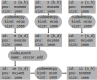
\includegraphics[width=0.5\textwidth]{figures/generated/dvdg.pdf}

        \end{minipage}

	\end{tabular}
\end{table}

Though it is generally possible to generate these dependence graphs by hand, it is not feasible for complicated applications.
Furthermore, as applications are updated, new models would have to be manually generated.
The proposed method described in this section would automate that process.

\section{Constructing the Dynamic Value Dependence Graph for Unmodified Applications}

Ideally, the DVDG would be generated from an unmodified application execution.
This ensures that the tool is as accessible to users as possible, and that it can work on closed-source applications
Unfortunately, the DVDG cannot rely on the application to advertise any helpful information about its behavior, and any relevant application state must be observed through its interaction with the operating system.
The proposed system (``apptracer'') leverages two tools available on the Linux platform: the CUDA Profiling Tools Interface (Section~\ref{sec:cupti} (CUPTI) and the Linux \texttt{LD\_PRELOAD} (Section~\ref{sec:ldpreload}) mechanism.

\texttt{apptracer} would use CUPTI to capture most CUDA-related information, and LD\_PRELOAD for everything else.
CUPTI allows a tool to provide a callback function that is invoked at every CUDA runtime or driver call, and also allows \texttt{apptracer} to collect any performance metrics the GPU exposes.
The callback function records relevant information, including the wall time when the CUDA runtime function is invoked, its arguments, and the device and stream associated with the call.
In this way, detailed information about data transfers from runtime functions can be reconstructed.
For example, allocations from \texttt{cudaMalloc} can be associated with pointers passed to \texttt{cudaMemcpy} to discover data transfers from host to device.

\texttt{apptracer} would use \texttt{LD\_PRELOAD} (Section~\ref{sec:ldpreload}) to intercept known API calls made by the application to shared libraries.
For example, \texttt{LD\_PRELOAD} could be used to observe file access, calls to CUDA libraries such as cuDNN or cuBLAS, network access, and system memory allocations.
The various kernel launches and allocations used by cuDNN and cuBLAS are already visible through CUPTI, but the known semantics of the higher-level cuBLAS and cuDNN calls allow for detailed edges to be added.

One challenge of \texttt{apptracer} is handling implicit data movement from three scenarios:
data moved from GPU global memory to arbitrary GPU kernels, implicit data movement between remote mappings, and implicit data movement through the unified memory system.
On supported systems, GPUs can directly access data that is on the host or other GPUs without making any CUDA runtime calls.
CUPTI allows the GPU to record detailed profiling information, but this affects program execution time and distorts the timeline.
A two-pass approach, once to collect accurate timeline information and another to capture more detailed information may be a solution.

Another challenge is for \texttt{apptracer} to infer which kernel arguments are pointers to allocations.
It may be possible for \texttt{apptracer} to examine the intermediate PTX representation of CUDA kernel code embedded in most CUDA binaries, and deduce some information about function signatures.

Once the application's use of CUDA is recorded, the next step would be to extend the graph to some view of activity on the CPU as well.
This could be accomplished through a variety of techniques.
The \texttt{LD\_PRELOAD} mechanism could be used to instrument popular libraries such as BLAS or MPI.
The operating system trace facilities strace~\cite{strace2018} for Linux, DTrace~\cite{dtrace2008} for MacOS, NtTrace~\cite{orr2014nttrace}, or Dr. Memory~\cite{bruening2001design}\cite{drmemory2018} for Windows could be used to track system calls and profile things such as file I/O or network interaction.
Tracking arbitrary function calls within an unmodified application may not be possible in the case of a binary without debug symbols.
Dynamic tracing tools like Intel's PIN~\cite{intel2012pin} can insert instrumentation code, but further work would be needed to determine the number of function arguments and their locations to recover their values.
For a cluster environment, it may be possible to generate distributed dependence graphs at each node, and then join them together by linking together information recorded about MPI calls.

\section{Combined Modeling}
\label{sec:modeling}

Finally, once system performance modeling is established, and application demands are recorded, joint performance modeling is possible, to tackle questions like
\begin{itemize}
    \item For a particular DVDG, what performance could we expect on a particular system?
    \item For a particular DVDG and a particular budget, what system configuration would perform best?
    \item For a particular DVDG, can the execution be rescheduled on a system to improve performance?
    \item How would changing link parameters or topology on a particular system affect application performance?
\end{itemize}
Answering these questions may require additional effort in open research challenges, such as task scheduling with placement-dependent communication costs, compute kernel performance estimation, and design space exploration.

\chapter{Related Work}
\label{ch:related}

\section{System Topology Enumeration / Hardware Models}

This work relies on and enhances an existing system topology enumeration tool, \texttt{hwloc}~\cite{broquedis2010hwloc}.
\texttt{hwloc} is designed around the expectation that current and next-generation systems are hierarchical.
This work uses \texttt{hwloc} to enumerate topology, but embeds the devices that \texttt{hwloc} discovers in a graph (Section~\ref{sec:hardware-enumeration}), which is a more general model of modern hardware systems.

Amaral et. al.~\cite{amaral2017topology} use a similar hardware graph, but their path costs are defined qualitatively, whereas this work proposes automating a quantitative cost that depends on the communication method used.
They also describe a topology-aware job placement strategy, but the problem considered is jobs on nodes in a cluster environment instead of computation tasks on GPUs.

\section{System Characterization}

Several prior benchmark suites strive to determine system parameters through microbenchmarking.
LMBench~\cite{mcvoy1996lmbench} is a benchmark designed to determine memory hierarchy parameters.
It includes a single-threaded memory bandwidth benchmark similar to the one included in this work.
It also includes cached I/O bandwidth measurements, a logical communication path that this work will be extended to explore.
P-Ray~\cite{duchateau2008p} is a benchmark suite designed to help guide performance autotuners.
It is designed to discover hardware parameters, such as L2 cache size.
Among other things, it extends LMBench's memory bandwidth microbenchmark to include multithreaded transfers.
Servet~\cite{gonzalez2010servet} goes a step further and includes a benchmark to determine communication costs between pairs of cores in the context of MPI.
It also attempts to analyze the results to establish which cores are equivalent from a communication perspective to simplify the benchmarking process.
BlackjackBench~\cite{danalis2012blackjackbench} benchmark suite designed to measure the observable performance parameters of a system as opposed to hardware paramters.
This work also takes the view that observable system parameters are what matters to application performance.
It focuses on memory hierarchy performance, but also includes a workload to measure communication bandwidth between pairs of CPU cores.
Liu et. al.~\cite{liu2004microbenchmark} take a microbenchmarking approach to evaluating high-speed cluster interconnects, including latency, uni- and bi-directional bandwidth, and host latency.
This work takes a similar approach or subsumes the communication microbenchmarking of this previous work, but extends it to many kinds of CUDA communication.

This work also proposes correlating microbenchmark performance directly with underlying hardware.
McCurdy and Vetter~\cite{mccurdy2010memphis} describe using performance counters to examine the NUMA abstraction and determine its mapping to the underlying hardware.
This work proposes to automate that analysis in Section~\ref{sec:logical-hardware-mapping}.

Some GPGPU benchmark suites also make an effort to characterize certain aspects of data-transfer performance.
The Scalable Heterogeneous Computing (SHOC) benchmark suite~\cite{danalis2010scalable} examines host-to-device and device-to-host data transfer on some PCIe-based systems.
This work examines a much broader set of CUDA communication capabilities.
It also examines the latency effect of data transfers conflicting with MPI message sending on the PCIe bus.
This contention effect is similar to some future contention characterization this work will be extended to.

Prior work has also specifically examined the communication performance effect of incorrect NUMA pinnings in multi-GPU systems.
Spafford, Meredith, and Vetter~\cite{spafford2011quantifying} show significant anisotropy and bandwidth degradation in PCIe bandwidth for incorrect NUMA pinnings. \todo{They also discuss some performance effect on applications and performance under contention}.

Limited prior work has examined performance of CUDA transfers specifically.
Landaverde et. al.~\cite{landaverde2014investigation}.
Li et. al~\cite{li2015evaluation} evaluate the unified memory system on several platforms, including a multi-CPU PCIe platform, and show around a 10\% performance penalty on some applications for Unified Memory.
They do not do any microbenchmarking, but observe that the unified memory system in CUDA 6.0 produced redundant transfers that were avoiding in the explicitly-managed code.
MGBench, a multi-GPU communication benchmark~\cite{bennun2016mgbench}, contains multi-GU microbenchmarks including scatter, direct access, and ring broadcast messages.
Ben-Nun et. al.~\cite{ben2017groute} examines direct-access transfers between GPUs.
They show the transfer rate of direct-access transfers between local GPUs, remote GPUs, and CPU/GPU transfers with various access patterns.
They observe that the performance is highly dependent on the access pattern.
Like this work, they discover that the transfer rate is highly correlated with the topological proximity of the devices.


\section{Using Communication Models}

Related works make use of the communication costs to make scheduling decisions.
MPIPP~\cite{chen2006mpipp} uses communication parameters in its process placement routine, but it gets them from the technical specification of the machine instead of measuring it.
Mercier~\cite{mercier2009towards} also uses communication parameters in its placement policy.
It determines the topology of the machine from the specification, and estimates the communication costs from that topology.

\section{NUMA / Multi-GPU APIs}

Prior work has made an effort to create NUMA-aware APIs, a possible future direction of this work.
Ben-Nun et. al.~\cite{ben2015memory} describes a multi-GPU partitioning framework for distributing parallel workloads on multi-GPU nodes according to their access patterns.
It provides a set of host and device APIs that describe containers and allow the framework to analyze kernels to determine access patters, to decide how to schedule underlying operations onto multiple GPUs.
Groute ~\cite{ben2017groute} propose parallel constructs for asynchronous multi-GPU programming.
The programming model involves describing the application communication pattern as a graph of communicating links and endpoints.
Section~\ref{sec:app-model} of this work describes the DVDG, which would be used to construct a similar application model for an exising application.

\todo{Umpire~\cite{beckingsale2018umpire}}.

\todo{https://github.com/woodun/9\_Microbenchmarks}.


\chapter{Conclusion}
\label{ch:conclusion}

This thesis examines the data-movement performance available to applications running on multi-GPU non-uniform memory access (NUMA) systems through a comprehensive series of microbenchmarks.
Three different systems are used as case studies: an IBM S822LC with two POWER8 CPUs and four P100 GPUs (Section~\ref{sec:s822lc}), an IBM AC922 with two POWER9 CPUs, four V100 GPUs, and NVLink 2.0 (Section~\ref{sec:ac922}), and an NVIDIA DGX-1 with two Intel (Section~\ref{sec:dgx1}), eight P100 GPUs, and hybrid PCIe and NVLink 1.0.
These three systems cover the common component for high-performance multi-GPU NUMA systems, with multiple CPUs, NVLink and PCIe 3.0 x16, and Pascal- or Volta-architecture GPUs.
The performance of the underlying hardware (Section~\ref{sec:interconnects}) in these systems is made available to applications through software abstractions (Section~\ref{sec:sys-abstraction}) like CUDA and numactl.
CUDA provides a variety of methods for moving data between system components (Section~\ref{sec:cuda}), where different choices have different performance effects due to different uses of the underlying hardware.

The core of this thesis are performance measurements of explicit(Chapter~\ref{ch:explicit}) and unified-memory (Chapter!\ref{ch:unified}) data-movement systems in CUDA.
These measurements are generated using a new series of microbenchmarks available at \texttt{https://github.com/rai-project/microbench}.
Generally, these benchmarks reveal that the CUDA method used to move data has a substantial impact on the actual performance available to the application, in some cases up to a $3x$ difference, as in the case of pinned transfers and coherence transfers.
When the data transfer method is simpler (pinned or prefetch transfers), performance is highly correlated with device affinity, but typically presents less anisotropic behavior.
This is because the underlying hardware link performance limits the overall throughput.
For more complicated transfer methods such as coherence, pageable transfers, or non-peer GPU-GPU transfers, performance tends to be more anisotropic but less correlated with device affinity.
The software overhead of managing these transfers tends to limit the performance more than the underlying links.
These results can be used to inform communication and allocation choices during application development, or allow an automated system to make the appropriate data-movement decision to provide the best performance.

In addition to the core performance measurements, this thesis also introduced a tool for enumerating the different communication hardware present in the system.
This tool is meant to serve as a foundational component of future systems research.
Any system that needs to make communication or scheduling performance decisions will need information about the underlying hardware that can be provided by this tool.
The system abstraction available through CUDA, the performance measurements, and the underlying hardware topology together provide the raw information for a detailed system model.

To complete the model, it will be necessary to automatically correlation communication abstractions to the underlying hardware (Section:~\ref{sec:map-underlying}).
This thesis also describes a corresponding application model (Section~\ref{sec:app-model}) that can be coupled with the system model.
Together these models should provide enough information to create an automatically-tuned high-performance heterogeneous memory management capability for multi-GPU NUMA systems.


%%%%%%%%%%%%%%%%%%%%%%%%%%%%%%%%%%%%%%%%%%%%%%%%%%%%%%%%%%%%%%%%%%%%%%%%%%%%%%%
% APPENDIX
%
\appendix
\begin{appendices}
	\chapter{Appendix A: Full Topologies}
\label{ch:full-topos}

\renewcommand\thefigure{A.\arabic{figure}} 

\begin{figure}[ht]
    \centering
    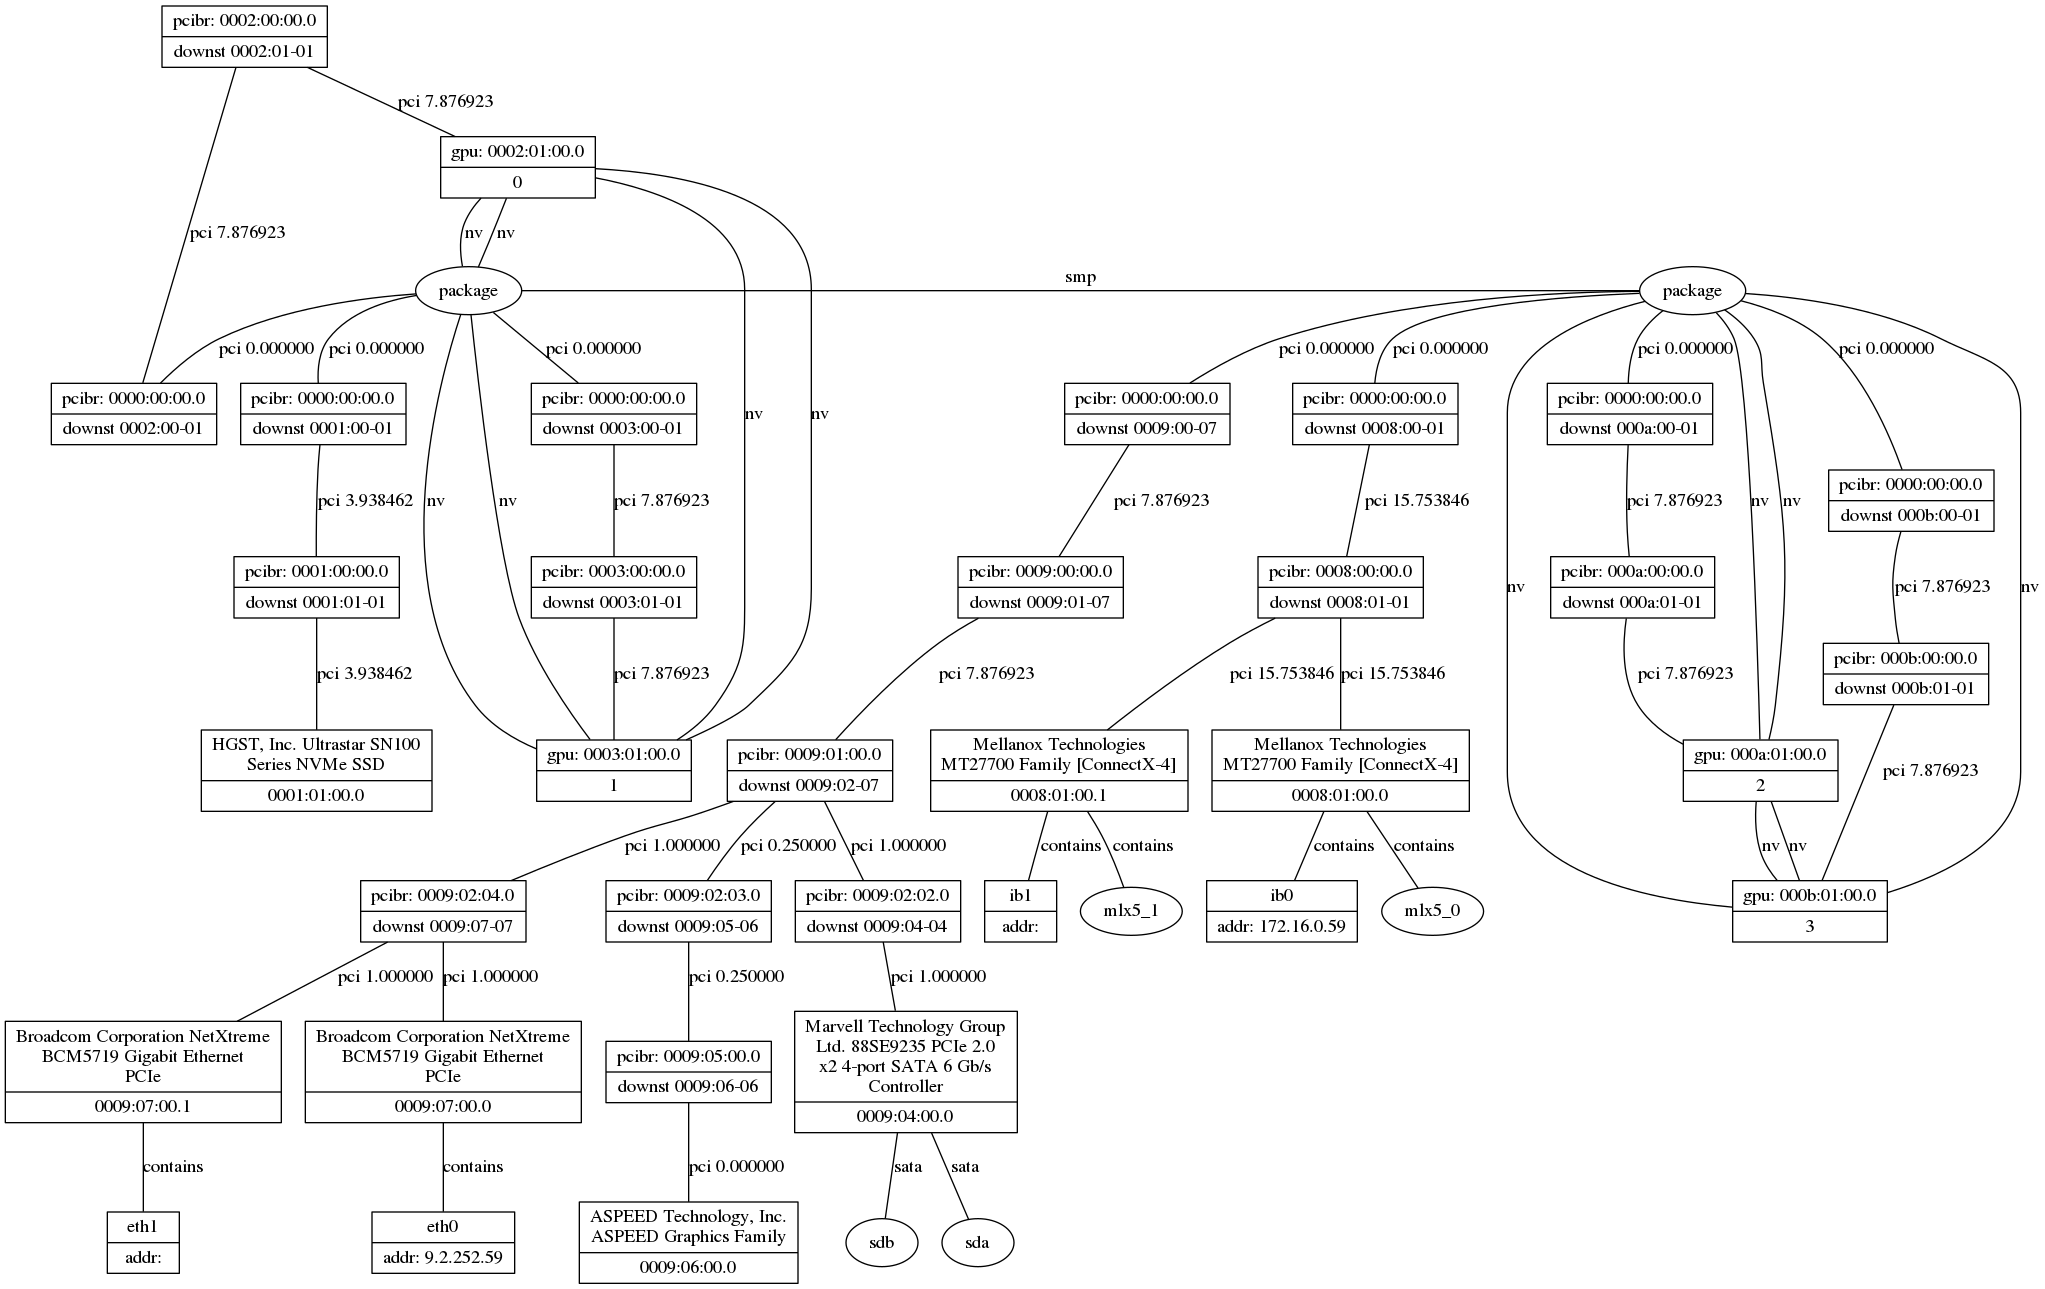
\includegraphics[width=\textwidth]{figures/topo-minsky-actual.png}
    \caption{S822LC discovered topology.}
    \label{fig:topo-minsky-actual}
\end{figure}

\begin{figure}[ht]
    \centering
    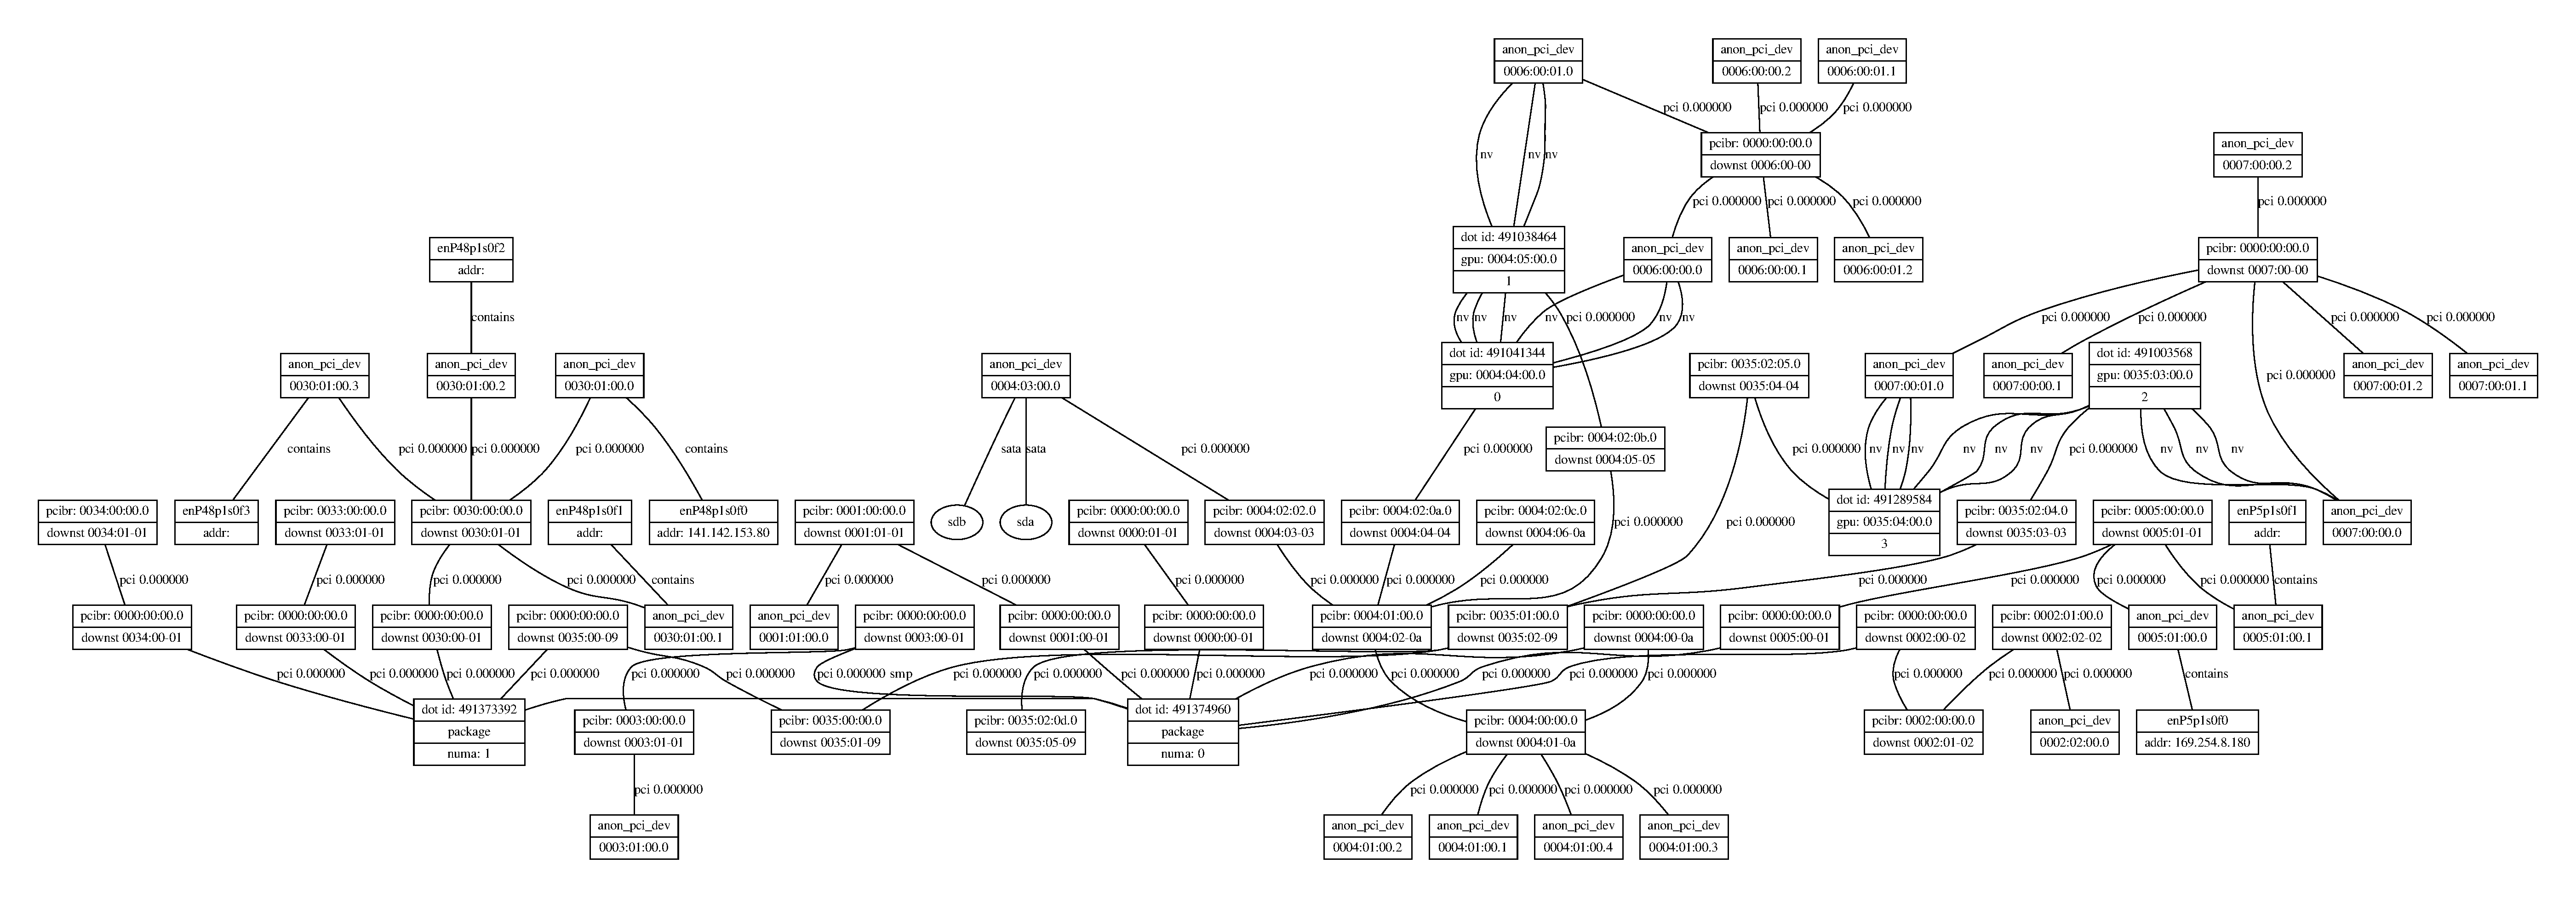
\includegraphics[width=\textwidth]{figures/topo-ac922-actual.pdf}
    \caption{AC922 discovered topology.}
    \label{fig:topo-ac922-actual}
\end{figure}

\begin{figure}[ht]
    \centering
    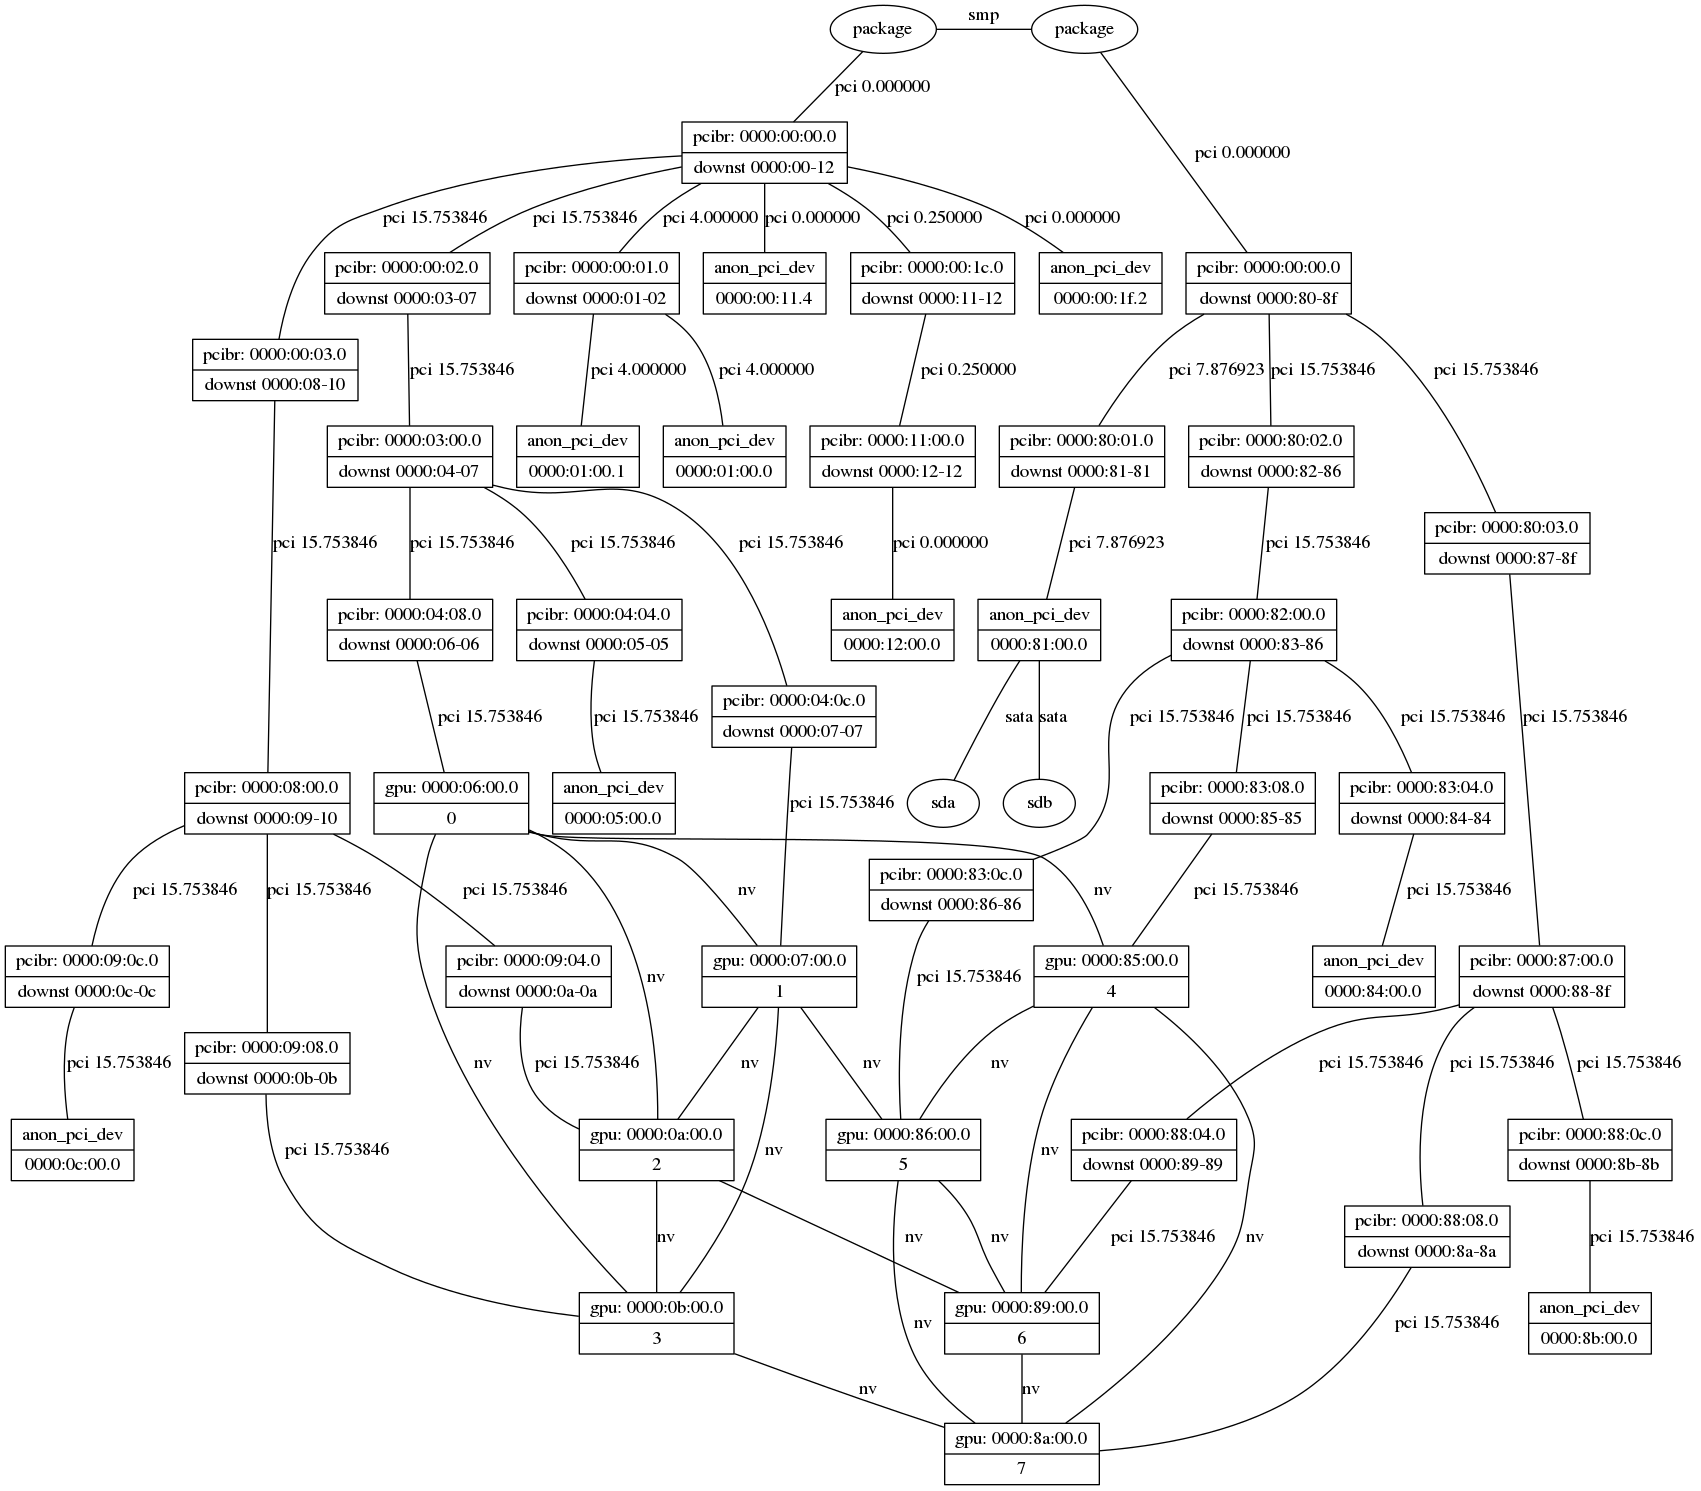
\includegraphics[width=\textwidth]{figures/topo-dgx1-actual.png}
    \caption{DGX-1 discovered topology.}
    \label{fig:topo-dgx-actual}
\end{figure}

	% \chapter{Complete Communication Data}
\label{ch:data}

\section{S822LC Pageable}

\begin{figure}[H]
    \centering
    \begin{subfigure}[b]{0.45\textwidth}
        \includegraphics[width=\textwidth]{figures/generated/minsky_pageable_cpu0-gpus.pdf}
        \caption{}
        \label{}
    \end{subfigure}
    ~
    \begin{subfigure}[b]{0.45\textwidth}
        \includegraphics[width=\textwidth]{figures/generated/minsky_pageable_cpu1-gpus.pdf}
        \caption{}
        \label{}
    \end{subfigure}
    \\
    \begin{subfigure}[b]{0.45\textwidth}
        \includegraphics[width=\textwidth]{figures/generated/minsky_pageable_gpus-cpu0.pdf}
        \caption{}
        \label{}
    \end{subfigure}
    ~
    \begin{subfigure}[b]{0.45\textwidth}
        \includegraphics[width=\textwidth]{figures/generated/minsky_pageable_gpus-cpu1.pdf}
        \caption{}
        \label{}
    \end{subfigure}
    \caption[\todo{short}]{\todo{long}}
    \label{fig:data-minsky-pageable}
\end{figure}

\section{S822LC Pinned}

\begin{figure}[H]
    \centering
    \begin{subfigure}[b]{0.45\textwidth}
        \includegraphics[width=\textwidth,draft]{figures/generated/minsky_pinned_cpu0-gpus.pdf}
        \caption{}
        \label{}
    \end{subfigure}
    ~
    \begin{subfigure}[b]{0.45\textwidth}
        \includegraphics[width=\textwidth,draft]{figures/generated/minsky_pinned_cpu1-gpus.pdf}
        \caption{}
        \label{}
    \end{subfigure}
    \\
    \begin{subfigure}[b]{0.45\textwidth}
        \includegraphics[width=\textwidth,draft]{figures/generated/minsky_pinned_gpus-cpu0.pdf}
        \caption{}
        \label{}
    \end{subfigure}
    ~
    \begin{subfigure}[b]{0.45\textwidth}
        \includegraphics[width=\textwidth,draft]{figures/generated/minsky_pinned_gpus-cpu1.pdf}
        \caption{}
        \label{}
    \end{subfigure}
    \caption[\todo{short}]{\todo{long}}
    \label{fig:data-minsky-pinned}
\end{figure}

\section{S822LC Write-Combined}

\begin{figure}[H]
    \centering
    \begin{subfigure}[b]{0.45\textwidth}
        \includegraphics[width=\textwidth,draft]{figures/generated/minsky_wc_cpu0-gpus.pdf}
        \caption{}
        \label{}
    \end{subfigure}
    ~
    \begin{subfigure}[b]{0.45\textwidth}
        \includegraphics[width=\textwidth,draft]{figures/generated/minsky_wc_cpu1-gpus.pdf}
        \caption{}
        \label{}
    \end{subfigure}
    \\
    \begin{subfigure}[b]{0.45\textwidth}
        \includegraphics[width=\textwidth,draft]{figures/generated/minsky_wc_gpus-cpu0.pdf}
        \caption{}
        \label{}
    \end{subfigure}
    ~
    \begin{subfigure}[b]{0.45\textwidth}
        \includegraphics[width=\textwidth,draft]{figures/generated/minsky_wc_gpus-cpu1.pdf}
        \caption{}
        \label{}
    \end{subfigure}
    \caption[\todo{short}]{\todo{long}}
    \label{fig:data-minsky-wc}
\end{figure}

\section{AC922 Pageable}

\begin{figure}[H]
    \centering
    \begin{subfigure}[b]{0.45\textwidth}
        \includegraphics[width=\textwidth,draft]{figures/generated/ac922_pageable_cpu0-gpus.pdf}
        \caption{}
        \label{}
    \end{subfigure}
    ~
    \begin{subfigure}[b]{0.45\textwidth}
        \includegraphics[width=\textwidth,draft]{figures/generated/ac922_pageable_cpu1-gpus.pdf}
        \caption{}
        \label{}
    \end{subfigure}
    \\
    \begin{subfigure}[b]{0.45\textwidth}
        \includegraphics[width=\textwidth,draft]{figures/generated/ac922_pageable_gpus-cpu0.pdf}
        \caption{}
        \label{}
    \end{subfigure}
    ~
    \begin{subfigure}[b]{0.45\textwidth}
        \includegraphics[width=\textwidth,draft]{figures/generated/ac922_pageable_gpus-cpu1.pdf}
        \caption{}
        \label{}
    \end{subfigure}
    \caption[\todo{short}]{\todo{long}}
    \label{fig:data-ac922-pageable}
\end{figure}

\section{AC922 Pinned}

\begin{figure}[H]
    \centering
    \begin{subfigure}[b]{0.45\textwidth}
        \includegraphics[width=\textwidth,draft]{figures/generated/ac922_pinned_cpu0-gpus.pdf}
        \caption{}
        \label{}
    \end{subfigure}
    ~
    \begin{subfigure}[b]{0.45\textwidth}
        \includegraphics[width=\textwidth,draft]{figures/generated/ac922_pinned_cpu1-gpus.pdf}
        \caption{}
        \label{}
    \end{subfigure}
    \\
    \begin{subfigure}[b]{0.45\textwidth}
        \includegraphics[width=\textwidth,draft]{figures/generated/ac922_pinned_gpus-cpu0.pdf}
        \caption{}
        \label{}
    \end{subfigure}
    ~
    \begin{subfigure}[b]{0.45\textwidth}
        \includegraphics[width=\textwidth,draft]{figures/generated/ac922_pinned_gpus-cpu1.pdf}
        \caption{}
        \label{}
    \end{subfigure}
    \caption[\todo{short}]{\todo{long}}
    \label{fig:data-ac922-pinned}
\end{figure}

\section{AC922 Write-Combined}

\begin{figure}[H]
    \centering
    \begin{subfigure}[b]{0.45\textwidth}
        \includegraphics[width=\textwidth,draft]{figures/generated/ac922_wc_cpu0-gpus.pdf}
        \caption{}
        \label{}
    \end{subfigure}
    ~
    \begin{subfigure}[b]{0.45\textwidth}
        \includegraphics[width=\textwidth,draft]{figures/generated/ac922_wc_cpu1-gpus.pdf}
        \caption{}
        \label{}
    \end{subfigure}
    \\
    \begin{subfigure}[b]{0.45\textwidth}
        \includegraphics[width=\textwidth,draft]{figures/generated/ac922_wc_gpus-cpu0.pdf}
        \caption{}
        \label{}
    \end{subfigure}
    ~
    \begin{subfigure}[b]{0.45\textwidth}
        \includegraphics[width=\textwidth,draft]{figures/generated/ac922_wc_gpus-cpu1.pdf}
        \caption{}
        \label{}
    \end{subfigure}
    \caption[\todo{short}]{\todo{long}}
    \label{fig:data-ac922-wc}
\end{figure}


\end{appendices}

\backmatter

%%%%%%%%%%%%%%%%%%%%%%%%%%%%%%%%%%%%%%%%%%%%%%%%%%%%%%%%%%%%%%%%%%%%%%%%%%%%%%%
% BIBLIOGRAPHY
%
\bibliographystyle{IEEE_ECE}

% Put references in BibTeX format in thesisrefs.bib.


\bibliography{thesisrefs}


\end{document}
\endinput
